\documentclass[../Thesis-IJspeert.tex]{subfiles}

\interfootnotelinepenalty=10000 %% Completely prevent breaking of footnotes

\begin{document}

\graphicspath{ {"Theory and Design of an Optical Resonator/figs/"} }
\pgfplotsset{table/search path={"Theory and Design of an Optical Resonator/data/"}}

\chapter{Theory and Design of an Optical Resonator}
\addtocontents{toc}{\vskip-6pt\par\noindent\protect\textcolor{gray75}{\protect\rule{\textwidth}{0.5pt}}\par}
\label{chap:TheoryandDesignofanOpticalResonator}

\section{Spectral properties}
A Fabry-Pérot resonator is an optical device that consists of two parallel, highly reflective mirrors separated by a fixed distance (see \autoref{fabryperot}).
\begin{figure}
	\centering
	\begin{tikzpicture}
	\vspace{0em}
	\centering
	\begin{groupplot}[group style={group name=my plots, group size=2 by 1,horizontal sep=2cm, vertical sep=2cm},height=4cm,width=6cm,no markers]
	\nextgroupplot
	[
	ylabel={},
	xmin=-2.5, xmax=2.5,
	ymin=-1.5, ymax=1.5,
	xticklabels={,,},
	yticklabels={,,},
	%legend pos=north west,
	ymajorgrids=false,
	xmajorgrids=false,
	grid style=dashed,
	axis lines=none,        % No axis lines
	tick style=none,        % No ticks
	xtick=\empty,           % No x-axis ticks
	ytick=\empty,           % No y-axis ticks
	xlabel={},              % No x-axis label
	ylabel={},              % No y-axis label
	%enlargelimits=true,     % Keeps the plot within the bounds
	clip=false,
	]
	
	\nextgroupplot
	[
	xlabel={$\sfrac{(\nu-\nu_0)}{\Delta \nu_\mathrm{FSR}}$},
	ylabel={$\sfrac{\lvert E_\mathrm{t}\rvert^2}{\,\lvert E_\mathrm{i} \rvert^2}$},
	ylabel style={yshift=0cm},
	xmin=-1.5, xmax=1.5,
	ymin=0, ymax=1.1,
	%xtick={0,1,2},
	%ytick={0,1,2,3},
	%yticklabels={$0$,$\sqrt{\frac{\lambda d}{\pi}}$,$2\sqrt{\frac{\lambda d}{\pi}}$,$3\sqrt{\frac{\lambda d}{\pi}}$},
	ymajorgrids=true,
	xmajorgrids=true,
	grid style=dashed,
	trig format plots=rad
	]
	
	\def\airy(#1,#2){{((1-#2)*(1-#2))/( pow((1-pow((#2*#2),(1/2))),2) + 4*pow((#2*#2),(1/2))*sin(pi*#1)*sin(pi*#1))}}
	
	\addplot [markgrijs, thick, domain=-1.5:1.5, samples=1000, name path = zerofive] (\x, {\airy(\x,0.5)});
	\addplot [markrood, thick, domain=-1.5:1.5, samples=1000, name path = zeronine] (\x, {\airy(\x,0.9)});
	\addplot [markgrijs!20,opacity=0, thick, domain=-1.5:1.5, samples=1000, name path = zero] (\x, 0);
	
	\addplot[markgrijs!20,opacity=0.5] fill between[of=zerofive and zeronine];
	\addplot[markrood!20,opacity=0.5] fill between[of=zeronine and zero];
	
	\fill [white] (axis cs:0.2, 0.45) rectangle (axis cs:0.8, 0.55);
	\fill [white] (axis cs:-0.75,0.4) rectangle (axis cs:-0.25,0.6);
	
	\draw[<->, markrood] (axis cs: -1, 1.03) -- (axis cs: 0, 1.03) node[midway, below] {\footnotesize $\Delta \nu_\mathrm{FSR}$};
	
	\draw[->, markrood] (axis cs: -1.2, 0.5) -- (axis cs: -1.02, 0.5);
	
	\draw[->, markrood] (axis cs: -0.8, 0.5) -- (axis cs: -0.98, 0.5) node[pos=0, right] {\footnotesize $\Delta \nu_\mathrm{A}$};
	
	\node[markgrijs, align=center, rotate=90] at (axis cs: 0.65, 0.6) {\footnotesize $R=0.5$};  
	\node[markrood, align=center, rotate=90] at (axis cs: 0.35, 0.6) {\footnotesize $R=0.9$};  
	%\node[markrood, align=center] at (axis cs: 0.5, 0.6) {\footnotesize $R=0.9$};  
	
	\draw[markrood] (axis cs: 0.35, 0.3) -- (axis cs: 0.085, 0.035);
	\draw[markgrijs] (axis cs: 0.65, 0.3) -- (axis cs: 0.75, 0.2);
	
	
	
	
	\end{groupplot}
	
	\begin{scope}[shift=(my plots c1r1.center)]
	
	% Define beam and mirror parameters
	\def\w0{0.5} % Beam waist
	\def\z0{1.5} % Rayleigh range
	\def\R{3} % Radius of the mirrors
	\def\mirrorsep{3} % distance between mirrors
	\def\angledeg{18}
	
	% Helper function for Gaussian beam radius
	\def\wbeam(#1){\w0*sqrt(1+pow((#1/\z0),2))}
	
	% Draw mirrors
	\def\centerarc[#1](#2)(#3:#4:#5)% [draw options] (center) (initial angle:final angle:radius)
	{ \draw[#1] ($(#2)+({#5*cos(#3)},{#5*sin(#3)})$) arc (#3:#4:#5); }
	
	\node[markgrijs, align=center, anchor=south] at (-\mirrorsep/2, 1.15) {\footnotesize $r_1$};
	\node[markgrijs, align=center, anchor=south] at (\mirrorsep/2, 1.15) {\footnotesize $r_2$};
	
	
	% cavity mirrors
	\draw[ultra thick, markgrijs] (-\mirrorsep/2-0.03, {1.0471975512}) -- (-\mirrorsep/2-0.03, {-1.0471975512});
	\draw[ultra thick, markgrijs] (\mirrorsep/2+0.03, {1.0471975512}) -- (\mirrorsep/2+0.03, {-1.0471975512});
	
	\draw[ultra thick, markgrijs] (-\mirrorsep/2-0.06, {1.0471975512}) -- (-\mirrorsep/2-0.06, {-1.0471975512});
	\draw[ultra thick, markgrijs] (\mirrorsep/2+0.06, {1.0471975512}) -- (\mirrorsep/2+0.06, {-1.0471975512});
	
	
	% horizontal beam in and outside cavity and labels
	\draw[markrood, thick, smooth, ->] (-3, 0.7) -- (2.3, 0.7) node[pos=1, above] {\footnotesize $E_\mathrm{t}$} node[pos=0, above] {\footnotesize $E_\mathrm{i}$}
	node[pos=0.37, above] {\footnotesize $it_1 E_\mathrm{i}$}
	node[pos=0.52, above, align=center] {\footnotesize $E_\mathrm{c}$};
	
	% labels for arcs
	\node[anchor=base, markrood] at (-0.23, 0.2) {\footnotesize $r_1 r_2 \mathrm{e}^{2i\phi}E_\mathrm{c}$};
	\node[anchor=base, markrood] at (-2.4, -0.1) {\footnotesize $r_1 E_\mathrm{i}$};
	\node[anchor=base, markrood] at (0.37, -0.43) {\footnotesize $r_2 \mathrm{e}^{i\phi} E_\mathrm{c}$};
	
	\draw[markrood, thick, smooth, ->] (0.5, -0.7) -- (-3, -0.7) node[pos=1, below] {\footnotesize $E_\mathrm{r}$};
	
	% arcs
	\begin{scope}[very thick,decoration={markings, mark=at position 0.5 with {\arrow{<}}}] 
	\centerarc[markrood, thick, smooth, postaction={decorate}](-2.59,0)(-90:90:0.7)
	\centerarc[markrood, thick, smooth, postaction={decorate}](0.5,0)(-90:90:0.7)
	\centerarc[markrood, thick, smooth, postaction={decorate}](-0.5,0)(-90+180:90+180:0.7)
	
	\end{scope}
	
	
	
	% cavity length
	\draw[<->, markgrijs] (-\mirrorsep/2, {-1*\wbeam(-\mirrorsep/2)-0.7}) -- (\mirrorsep/2, {-1*\wbeam(-\mirrorsep/2)-0.7}) node[midway, below] {\footnotesize $d$};
	
	\draw[dashed, markgrijs] (-\mirrorsep/2, {-1*\wbeam(-\mirrorsep/2)-0.7}) -- (-\mirrorsep/2, {-1.0471975512});
	\draw[dashed, markgrijs] (\mirrorsep/2, {-1*\wbeam(-\mirrorsep/2)-0.7}) -- (\mirrorsep/2, {-1.0471975512});
	
	\end{scope}
	
	\end{tikzpicture}
	\caption[Schematic of a Fabry-Pérot resonator and its transmission characteristics]{Schematic of a Fabry-Pérot resonator (left) and its transmission characteristics (right). The cavity consists of two mirrors with reflectivities $r_1$ and $r_2$, separated by a distance $d$. Incident light of amplitude $E_\mathrm{i}$ undergoes multiple reflections, which leads to interference within the cavity, which is either constructive or destructive depending on the round-trip phase shift $2\phi$. On the right, the normalised transmitted intensity $\sfrac{\lvert E_\mathrm{t}\rvert^2}{\,\lvert E_\mathrm{i}\rvert^2}$ is plotted as a function of normalised frequency detuning $\sfrac{(\nu - \nu_0)}{\Delta \nu_{\mathrm{FSR}}}$ from resonance ($\nu_0$) for two values of $R=r_1^2=r_2^2$. The free spectral range $\Delta \nu_{\mathrm{FSR}}$ is the spacing between adjacent resonances, while $\Delta \nu_A$ denotes the FWHM linewidth of the transmission profile that follows an Airy distribution.}
	\label{fabryperot} 
\end{figure}
Light entering the resonator undergoes multiple reflections between the mirrors, causing constructive or destructive interference. This gives rise to resonator modes at certain frequencies and a characteristic lineshape of the transmitted light, which will be discussed throughout the following sections.

\subsection{Resonance frequencies}
Whether the condition for constructive interference is satisfied depends on the round-trip phase accumulated by the light propagating inside the resonator. For light entering at a frequency of $\nu$, this round-trip phase shift (written as $2\phi$) equals twice the single-pass phase shift $\phi$, which can be expressed in terms of the wavenumber $k$ and the mirror separation $d$ as
\begin{align}
\label{phiairy}
\phi=kd=\pi\nu\frac{2d}{c}=\pi\frac{\nu}{\Delta\nu_\mathrm{FSR}}\,,
\end{align}
where $c$ denotes the speed of light in vacuum and $\Delta\nu_\mathrm{FSR}:=\sfrac{c}{2d}$, a quantity that is referred to as the free spectral range of the resonator. Resonances occur when light interferes constructively with itself upon a round-trip inside the cavity. This corresponds to frequencies for which the round-trip phase shift $2\phi$ equals a multiple of $2\pi$:
\begin{align}
\label{rescondition}
2\phi=2\pi q,\quad q \in \Z\,.
\end{align}
The integer $q$ is referred to as the mode index and labels the resonance that occurs at a frequency of $\nu_q=q\Delta\nu_\mathrm{FSR}$ or a wavenumber of $k_q=2\pi q \Delta\nu_\mathrm{FSR}/c$. It follows that the free spectral range $\Delta\nu_\mathrm{FSR}$ as defined earlier can be interpreted as the frequency spacing between two adjacent modes, as can be seen in \autoref{fabryperot}.

\subsection{Lineshape and finesse}
In this section, we derive the lineshape of the Fabry-Pérot resonator as shown in \autoref{fabryperot} by considering the transmitted field intensity ${\lvert E_\mathrm{t}\rvert^2}$ relative to the incident field intensity ${\lvert E_\mathrm{i}\rvert^2}$. This is done by relating both $ E_\mathrm{i}$ and $ E_\mathrm{t}$ to $ E_\mathrm{c}$, which is the steady-state amplitude of the field circulating inside the resonator. To find these relations, we assume that the optical thickness of the mirrors (lossless, thin dielectric slabs) is an odd number of quarter wavelengths. In addition, we consider the waves at separate reference planes that are located on opposite sides of this slab and are thus separated by the mirror thickness. In this case, the amplitude reflection coefficients from both sides of the mirror are symmetric and purely real (denoted $r_1$ and $r_2$). The amplitude transmission factors, however, acquire an additional phase shift of $\sfrac{\pi}{2}$ and can thus be written as $it_1$ and $it_2$, where $t_i\in \mathbb{R}$ and $r_i^2+t_i^2=1$ for $i\in \{ 1,2\}$. With these conventions, we can write
\begin{align}
\begin{split}
&E_\mathrm{t}= it_2 \mathrm{e}^{i\phi} E_\mathrm{c} \implies \frac{E_\mathrm{t}}{E_\mathrm{c}} = it_2 \mathrm{e}^{i\phi}\\
&E_\mathrm{c}= it_1 E_\mathrm{i} + r_1 r_2 \mathrm{e}^{2i\phi} E_\mathrm{c} \implies \frac{E_\mathrm{c}}{E_\mathrm{i}} = \frac{it_1}{1-r_1 r_2 \mathrm{e}^{2i\phi}} \,.
\end{split}
\end{align}
Using these results, we can calculate the calculate the normalised transmitted intensity as
\begin{align}
\label{airy}
\frac{\lvert E_\mathrm{t}\rvert^2}{\lvert E_\mathrm{i}\rvert^2} = \frac{\lvert -t_1 t_2 \mathrm{e}^{i\phi}\rvert^2}{\lvert 1-r_1 r_2\mathrm{e}^{2i\phi}\rvert^2}=\frac{(1-R_1)(1-R_2)}{\left(1-\sqrt{R_1R_2}\,\right)^2 + 4\sqrt{R_1R_2}\sin^2(\phi)}\,,
\end{align}
written in terms of the intensity reflectivities $R_1=r_1^2$ and $R_2=r_2^2$ of the left and right mirror, respectively. The form in \autoref{airy} represents the Airy distribution and is shown in \autoref{fabryperot} for two different values of $R=R_1=R_2$. A useful quantity in the context of optical resonators is finesse, which is a measure of how narrow the resonances are in relation to the free spectral range (higher finesse corresponding to narrower lines). The width $\Delta \nu_\mathrm{A}$ of a peak in the transmission profile of the resonator is defined as the full width at half maximum (FWHM), which can be derived from \autoref{airy} considering the phase change $\Delta \phi$ over which the Airy distribution drops from its maximum where $\sin^2(\phi)=0$ to half its maximum value:
\begin{align}
\Delta\phi=\arcsin{\frac{1-\sqrt{R_1R_2}}{2\sqrt[4]{R_1R_2}}}\,.
\end{align}
Since $2\Delta\phi={\pi\Delta\nu_\mathrm{A}}/{\Delta\nu_\mathrm{FSR}}$ (see \autoref{phiairy}), we can calculate the finesse $\mathcal{F}$ as
\begin{align}
\mathcal{F}:=\frac{\Delta_\mathrm{FSR}}{\Delta\nu_\mathrm{A}}=\frac{\pi}{2}\left(\arcsin{\frac{1-\sqrt{R_1R_2}}{2\sqrt[4]{R_1R_2}}}\right)^{-1}\,.
\end{align}
Note that the finesse is independent of the resonator length and is instead fully determined by the properties of the mirrors. For values of $\phi$ close to the nearest integer multiple of $\phi$, or more precisely $\min\{\lvert \phi \bmod \pi \rvert, \lvert \phi \bmod \pi - \pi\rvert\} \ll 1$, we can approximate $\sin^2(\phi)\approx\phi^2$ in \autoref{airy}, which yields
\begin{align}
\label{approxfinesse}
\mathcal{F}\approx \pi \frac{\sqrt[4]{R_1R_2}}{1-\sqrt{R_1R_2}}\,.
\end{align}
In the case of identical mirrors ($R_1=R_2=R$), \autoref{approxfinesse} reduces to $\mathcal{F}\approx \pi{\sqrt{R}}/(1-R)$.

\section{Transverse modes}
In a Fabry-Pérot resonator, the standing wave patterns that form between the mirrors are not limited to a single uniform distribution across the transverse (perpendicular to the optical axis) plane but can exhibit various spatial intensity distributions, known as transverse modes. Each transverse mode corresponds to a specific solution of the paraxial Helmholtz equation within the resonator. The most fundamental modes are Gaussian, which have a single intensity peak centred on the optical axis. Higher-order transverse modes, such as Hermite-Gaussian, Laguerre-Gaussian, and Ince-Gaussian modes, exhibit increasingly complex intensity profiles with distinct nodal structures. These modes differ not only in their spatial energy distributions but also in their resonance frequencies due to their transverse confinement, a phenomenon known as transverse mode spacing. Throughout this section, we will discuss the paraxial Helmholtz equation that governs these solutions, which is followed by an analysis of Gaussian and higher-order modes.
\subsection{The paraxial Helmholtz equation}
The paraxial Helmholtz equation provides a fundamental framework for describing the propagation of light in optical systems where the beam divergence is small, and the paraxial approximation holds. Its solutions form the basis for understanding the transverse modes of Fabry-Pérot resonators, including Gaussian beams and their higher-order generalisations. The derivation and key properties of these solutions are presented in this section. We start from the Helmholtz equation, which reads
\begin{align}
\label{Helmholtz}
\left(\nabla^2 + k^2\right) E_0^{(+)}(\vec{r}\,)=0\,,
\end{align}
written in terms of the wavenumber $k$ and the complex electric field amplitude $E_0^{(+)}(\vec{r}\,)$ as defined in \autoref{Efield}. For a plane wave travelling along the $z$ direction, we can write the complex electric field amplitude as
\begin{align}
E_0^{(+)}(\vec{r}\,)=u(\vec{r}\,)\mathrm{e}^{ikz}\,
\end{align}
where $u(\vec{r}\,)$ represents the complex transverse profile. In the paraxial approximation, this complex envelope varies sufficiently slowly with propagation distance $z$, such that the following inequalities are satisfied:
\begin{align}
\left\lvert \frac{\partial^2 u}{\partial z^2} \right\rvert \ll  \left\lvert 2k \frac{\partial u}{\partial z}\right\rvert , \left\lvert \frac{\partial^2 u}{\partial x^2} \right\rvert, \left\lvert \frac{\partial^2 u}{\partial y^2} \right\rvert \,.
\end{align}
Under these conditions, \autoref{Helmholtz} simplifies to the paraxial Helmholtz equation
\begin{align}
\label{paraxialHelmholtz}
\Delta_\perp u(\vec{r}\,)+2ik\frac{\partial}{\partial z}u(\vec{r}\,)=0\,,
\end{align}
where $\Delta_\perp={\partial^2}/{\partial x^2} + {\partial^2}/{\partial x^2}$ is the transverse Laplacian operator.
\subsection{Gaussian modes}
The Gaussian beam\footnote{With an intensity profile as given in \autoref{laser}.} is the fundamental solution to the paraxial Helmholtz equation and represents the simplest transverse mode of optical resonators with a spatially localised intensity profile. It can be written in cylindrical coordinates as \cite{Saleh1991}
\begin{align}
\label{gaussianmode}
u(r, \phi, z) = \frac{w_0}{w(z)}\exp{\frac{-r^2}{w^2(z)}}\exp{i\left( kz + \frac{kr^2}{2R_\mathrm{c}(z)} - \Psi(z)\right)}\,,
\end{align}
in terms of the waist radius $w_0$, the beam radius $w(z)$ at a distance $z$ and Rayleigh length $z_\mathrm{R}$, which were given in \autoref{dipoleforce}. We have furthermore introduced the wavefront curvature radius $R_\mathrm{c}(z)=z(1+(\sfrac{z_\mathrm{R}}{z})^2)$ and the Guoy phase $\Psi(z)=\arctan\left(\sfrac{z}{z_\mathrm{R}}\right)$. The expression for $R_\mathrm{c}(z)$ illustrates how the wavefront curvature becomes spherical away from the beam waist and flattens as $z \to 0$. The Gouy phase accounts for the additional phase accumulated by a focused beam and increases smoothly from $\sfrac{-\pi}{2}$ to $\sfrac{\pi}{2}$ as the beam propagates through the focus. In the context of optical resonators, it is important to note that Gaussian beams constitute solutions to the paraxial Helmholtz equation subject to the boundary conditions imposed by a pair of spherical mirrors in a Fabry-Pérot cavity. This is due to the fact that a reflected Gaussian beam will retrace itself as long as the curvature of its wavefront matches that of the mirror. For a pair of concave, spherical mirrors separated by a distance $d$ and matching the Gaussian wavefront at their respective positions, the beam can, through repeated reflections, exist self-consistently within this optical resonator. Under the additional condition that the phase retraces itself upon reflection, the Gaussian beam is said to be a mode of the resonator. For a Gaussian mode in a symmetric spherical-mirror resonator (with mirror radii of curvature\footnote{A negative radius of curvature corresponds to a concave mirror. We therefore define the mirror radii of curvature as $R_{\mathrm{c},1}=R_\mathrm{c}(\sfrac{-d}{2})$ and $R_{\mathrm{c},2}=-R_\mathrm{c}(\sfrac{d}{2})$ in terms of the wavefront curvature radius $R_\mathrm{c}(z)$. For mirrors of equal curvature we write $R_{\mathrm{c},1}=R_{\mathrm{c},2}= R_\mathrm{c}$.} $R_{\mathrm{c},1}=R_{\mathrm{c},2}=-\lvert R_\mathrm{c} \rvert$ for concave mirrors), the beam waist $w_0$ and beam radii $w_1$ and $w_2$ at the mirror positions ($w_1=w(\sfrac{-d}{2})$ and $w_2=w(\sfrac{d}{2})$) can be calculated from the following relations:
\begin{align}
\label{waisteqs}
\begin{split}
&w_0^2 = \frac{\lambda d}{2\pi}\sqrt{2\frac{\lvert R_\mathrm{c} \rvert}{d} - 1}\\
&w_1^2 = w_2^2 = \frac{\lambda d}{\pi} \frac{1}{\sqrt{\sfrac{d}{\lvert R_\mathrm{c} \rvert}\left( 2 - \sfrac{d}{\lvert R_\mathrm{c} \rvert} \right)}}\,.
\end{split}
\end{align}
To avoid unconfined solutions to the paraxial Helmholtz equation, which is to prevent diverging beam radii in \autoref{waisteqs}, the modulus of the mirror radius of curvature $\lvert R_\mathrm{c} \rvert$ and mirror separation $d$ must satisfy the confinement criterion:
\begin{align}
0 \le \frac{d}{\lvert R_\mathrm{c} \rvert} \le 2\,.
\end{align}
\autoref{beamradiusincavity} illustrates the behaviour of the beam radius inside a symmetric optical resonator for different values of $\sfrac{d}{\lvert R_\mathrm{c} \rvert}$.
\begin{figure}[t]
	\centering
	\begin{tikzpicture}
	\vspace{0em}
	\centering
	\begin{groupplot}[group style={group name=my plots, group size=2 by 2,horizontal sep=4cm, vertical sep=2cm},height=4cm,width=4cm,no markers]
	\nextgroupplot
	[
	ylabel={},
	xmin=-2.5, xmax=2.5,
	ymin=-1.5, ymax=1.5,
	xticklabels={,,},
	yticklabels={,,},
	%legend pos=north west,
	ymajorgrids=false,
	xmajorgrids=false,
	grid style=dashed,
	axis lines=none,        % No axis lines
	tick style=none,        % No ticks
	xtick=\empty,           % No x-axis ticks
	ytick=\empty,           % No y-axis ticks
	xlabel={},              % No x-axis label
	ylabel={},              % No y-axis label
	%enlargelimits=true,     % Keeps the plot within the bounds
	clip=false,
	]
	
	
	\nextgroupplot
	[
	ylabel={},
	xmin=-2.5, xmax=2.5,
	ymin=-1.5, ymax=1.5,
	xticklabels={,,},
	yticklabels={,,},
	%legend pos=north west,
	ymajorgrids=false,
	xmajorgrids=false,
	grid style=dashed,
	axis lines=none,        % No axis lines
	tick style=none,        % No ticks
	xtick=\empty,           % No x-axis ticks
	ytick=\empty,           % No y-axis ticks
	xlabel={},              % No x-axis label
	ylabel={},              % No y-axis label
	%enlargelimits=true,     % Keeps the plot within the bounds
	clip=false,
	]
	
	
	\nextgroupplot
	[
	ylabel={},
	xmin=-2.5, xmax=2.5,
	ymin=-1.5, ymax=1.5,
	xticklabels={,,},
	yticklabels={,,},
	%legend pos=north west,
	ymajorgrids=false,
	xmajorgrids=false,
	grid style=dashed,
	axis lines=none,        % No axis lines
	tick style=none,        % No ticks
	xtick=\empty,           % No x-axis ticks
	ytick=\empty,           % No y-axis ticks
	xlabel={},              % No x-axis label
	ylabel={},              % No y-axis label
	%enlargelimits=true,     % Keeps the plot within the bounds
	clip=false,
	]
	
	\nextgroupplot
	[
	xlabel={$\sfrac{d}{\lvert R_\mathrm{c} \rvert}$},
	ylabel={Beam radius $w$},
	ylabel style={markrood},
	yticklabel style=markrood,
	every y tick/.style={markrood},
	xmin=0, xmax=2,
	ymin=0, ymax=2,
	xtick={0,1,2},
	ytick={0,1,2,3},
	yticklabels={$0$,$\sqrt{\frac{\lambda d}{\pi}}$,$2\sqrt{\frac{\lambda d}{\pi}}$,$3\sqrt{\frac{\lambda d}{\pi}}$},
	ymajorgrids=true,
	xmajorgrids=true,
	grid style=dashed,
	axis line style=transparent,
	ytick pos=left,
	]
	
	\addplot [markrood, domain=0:2, samples=1000, thick] (x, {2^(-1/2)*(2/x-1)^(1/4)});
	\addplot [markrood, domain=0:2, samples=1000, thick] (x, {(1/(x*(2-x)))^(1/4)});
	
	\node[markrood] at (axis cs: 0.6, 0.65) {\footnotesize $w_0$}; 
	\node[markrood] at (axis cs: 1.3, 1.5) {\footnotesize $w_1=w_2$}; 
	
	\end{groupplot}
	
	\begin{groupplot}[group style={group name=my second plots, group size=2 by 2,horizontal sep=4cm, vertical sep=2cm},height=4cm,width=4cm,no markers]
	\nextgroupplot
	[
	ylabel={},
	xmin=-2.5, xmax=2.5,
	ymin=-1.5, ymax=1.5,
	xticklabels={,,},
	yticklabels={,,},
	%legend pos=north west,
	ymajorgrids=false,
	xmajorgrids=false,
	grid style=dashed,
	axis lines=none,        % No axis lines
	tick style=none,        % No ticks
	xtick=\empty,           % No x-axis ticks
	ytick=\empty,           % No y-axis ticks
	xlabel={},              % No x-axis label
	ylabel={},              % No y-axis label
	%enlargelimits=true,     % Keeps the plot within the bounds
	clip=false,
	]
	
	
	\nextgroupplot
	[
	ylabel={},
	xmin=-2.5, xmax=2.5,
	ymin=-1.5, ymax=1.5,
	xticklabels={,,},
	yticklabels={,,},
	%legend pos=north west,
	ymajorgrids=false,
	xmajorgrids=false,
	grid style=dashed,
	axis lines=none,        % No axis lines
	tick style=none,        % No ticks
	xtick=\empty,           % No x-axis ticks
	ytick=\empty,           % No y-axis ticks
	xlabel={},              % No x-axis label
	ylabel={},              % No y-axis label
	%enlargelimits=true,     % Keeps the plot within the bounds
	clip=false,
	]
	
	
	\nextgroupplot
	[
	ylabel={},
	xmin=-2.5, xmax=2.5,
	ymin=-1.5, ymax=1.5,
	xticklabels={,,},
	yticklabels={,,},
	%legend pos=north west,
	ymajorgrids=false,
	xmajorgrids=false,
	grid style=dashed,
	axis lines=none,        % No axis lines
	tick style=none,        % No ticks
	xtick=\empty,           % No x-axis ticks
	ytick=\empty,           % No y-axis ticks
	xlabel={},              % No x-axis label
	ylabel={},              % No y-axis label
	%enlargelimits=true,     % Keeps the plot within the bounds
	clip=false,
	]
	
	\nextgroupplot
	[
	%xlabel={$\sfrac{d}{\lvert R \rvert}$},
	ylabel={Rayleigh length $z_0$},
	ylabel style={markgrijs},
	yticklabel style=markgrijs,
	every y tick/.style={markgrijs},
	ytick pos=right,
	xmin=0, xmax=2,
	ymin=0, ymax=2,
	xtick={0,1,2},
	ytick={0,1,2},
	yticklabels={$0$,$\frac{d}{2}$,$d$},
	ymajorgrids=false,
	xmajorgrids=false,
	grid style=dashed,
	xtick=\empty,
	]
	
	\addplot [markgrijs, domain=0:2, samples=1000, thick] (x, {(2/x-1)^(1/2)});
	
	
	
	\end{groupplot}
	
	
	
	\begin{scope}[shift=(my plots c1r1.center)]
	
	% Define beam and mirror parameters
	\def\w0{0.5} % Beam waist
	\def\z0{1.5} % Rayleigh range
	\def\R{3} % Radius of the mirrors
	\def\mirrorsep{3} % distance between mirrors
	\def\angledeg{18}
	
	% Helper function for Gaussian beam radius
	\def\wbeam(#1){\w0*sqrt(1+pow((#1/\z0),2))}
	
	% Draw mirrors
	\def\centerarc[#1](#2)(#3:#4:#5)% [draw options] (center) (initial angle:final angle:radius)
	{ \draw[#1] ($(#2)+({#5*cos(#3)},{#5*sin(#3)})$) arc (#3:#4:#5); }
	
	% Dashed lines for mirror radius
	%\draw[->, dashed, markgrijs] (-\mirrorsep/2,0) -- ({-\mirrorsep/2+\R*cos(\angledeg)}, {\R*sin(\angledeg)})
	%    node[pos=0.85, anchor=south east, align=center] {\footnotesize $\lvert R \rvert$};
	%\draw[->, dashed, markgrijs] (\mirrorsep/2,0) -- ({\mirrorsep/2+\R*cos(\angledeg+180)}, {-\R*sin(\angledeg+180)})
	%    node[pos=0.85, anchor=south west, align=center] {\footnotesize $\lvert R \rvert$};
	
	\node[markgrijs, align=center, anchor=south] at (-\mirrorsep/2, 1.0471975512) {\footnotesize $\lvert R_\mathrm{c} \rvert \rightarrow\infty$};
	\node[markgrijs, align=center, anchor=south] at (\mirrorsep/2, 1.0471975512) {\footnotesize $\lvert R_\mathrm{c} \rvert \rightarrow\infty$};
	
	% Axes
	\draw[->] (2.19,0) -- (2.5,0) node[below right] {$z$};
	\draw[] (-2.5,0) -- (-2.2,0);
	\draw[] (-1.98,0) -- (-0.4,0);
	\draw[] (-0.18,0) -- (1.97,0);
	\draw[->] (0,-1.3) -- (0,1.3) node[above] {$w(z)$};
	
	% Gaussian beam shaded region
	\begin{scope}
	\clip (-\mirrorsep, -1.5) rectangle (\mirrorsep, 1.5); % Clip region for beam shading
	\fill[markrood!20,opacity=0.5] plot[domain=-1.5:1.5,smooth] (\x, {1.0471975512})
	-- plot[domain=1.5:-1.5,smooth] (\x, {-1.0471975512}) -- cycle;
	\end{scope}
	
	% Gaussian beam outline
	%\draw[markrood, thick, smooth] plot[domain=-1.5:1.5] (\x, {\wbeam(\x)});
	%\draw[markrood, thick, smooth] plot[domain=-1.5:1.5] (\x, {-\wbeam(\x)});
	
	% cavity mirrors
	\draw[ultra thick, markgrijs] (-\mirrorsep/2-0.03, {1.0471975512}) -- (-\mirrorsep/2-0.03, {-1.0471975512});
	\draw[ultra thick, markgrijs] (\mirrorsep/2+0.03, {1.0471975512}) -- (\mirrorsep/2+0.03, {-1.0471975512});
	
	\draw[ultra thick, markgrijs] (-\mirrorsep/2-0.06, {1.0471975512}) -- (-\mirrorsep/2-0.06, {-1.0471975512});
	\draw[ultra thick, markgrijs] (\mirrorsep/2+0.06, {1.0471975512}) -- (\mirrorsep/2+0.06, {-1.0471975512});
	
	% Beam waist label
	\draw[<->, markrood] (-0, 1.0471975512) -- (-0, -1.0471975512) node[pos=0.5, left, anchor=south, rotate=90] {\footnotesize $2w_0\rightarrow\infty$};
	% Beam radius at mirror label
	\draw[<->, markrood] ({-\mirrorsep/2-0.3}, {1.0471975512}) -- ({-\mirrorsep/2-0.3}, {-1.0471975512}) node[pos=0.5, left, anchor=south, rotate=90] {\footnotesize $2w_1\rightarrow\infty$};
	%\draw[markrood, dashed] ({-\mirrorsep/2-0.3}, {\wbeam(-\mirrorsep/2)}) -- (-\mirrorsep/2, {\wbeam(-\mirrorsep/2)});
	%\draw[markrood, dashed] ({-\mirrorsep/2-0.3}, {-1*\wbeam(-\mirrorsep/2)}) -- (-\mirrorsep/2, {-1*\wbeam(-\mirrorsep/2)});
	
	% Beam radius at mirror label
	\draw[<->, markrood] ({\mirrorsep/2+0.3}, {1.0471975512}) -- ({\mirrorsep/2+0.3}, {-1.0471975512}) node[pos=0.5, right, anchor=north, rotate=90] {\footnotesize $2w_2\rightarrow\infty$};
	%\draw[markrood, dashed] ({\mirrorsep/2+0.3}, {\wbeam(-\mirrorsep/2)}) -- (\mirrorsep/2, {\wbeam(-\mirrorsep/2)});
	%\draw[markrood, dashed] ({\mirrorsep/2+0.3}, {-1*\wbeam(-\mirrorsep/2)}) -- (\mirrorsep/2, {-1*\wbeam(-\mirrorsep/2)});
	
	% Rayleigh range label
	%\draw[<->, markrood] (0, 0) -- (\z0, 0) node[midway, below] {\footnotesize $z_0$};
	
	% cavity length
	\draw[<->, markgrijs] (-\mirrorsep/2, {-1*\wbeam(-\mirrorsep/2)-0.7}) -- (\mirrorsep/2, {-1*\wbeam(-\mirrorsep/2)-0.7}) node[midway, below] {\footnotesize $d$};
	
	\draw[dashed, markgrijs] (-\mirrorsep/2, {-1*\wbeam(-\mirrorsep/2)-0.7}) -- (-\mirrorsep/2, {-1.0471975512});
	\draw[dashed, markgrijs] (\mirrorsep/2, {-1*\wbeam(-\mirrorsep/2)-0.7}) -- (\mirrorsep/2, {-1.0471975512});
	
	\node[align=center, anchor=center] at (0.75, -1.0471975512/2) {\footnotesize $\sfrac{d}{\lvert R \rvert}= 0$};
	
	\end{scope}
	
	\begin{scope}[shift=(my plots c2r1.center)]
	
	% Define beam and mirror parameters
	\def\w0{0.5} % Beam waist
	\def\z0{1.5} % Rayleigh range
	\def\R{3} % Radius of the mirrors
	\def\mirrorsep{3} % distance between mirrors
	\def\angledeg{20}
	
	% Helper function for Gaussian beam radius
	\def\wbeam(#1){\w0*sqrt(1+pow((#1/\z0),2))}
	
	% Draw mirrors
	\def\centerarc[#1](#2)(#3:#4:#5)% [draw options] (center) (initial angle:final angle:radius)
	{ \draw[#1] ($(#2)+({#5*cos(#3)},{#5*sin(#3)})$) arc (#3:#4:#5); }
	
	% Dashed lines for mirror radius
	\draw[->, dashed, markgrijs] (-\mirrorsep/2,0) -- ({-\mirrorsep/2+\R*cos(\angledeg)}, {\R*sin(\angledeg)})
	node[pos=0.85, anchor=south east, align=center] {\footnotesize $\lvert R_\mathrm{c} \rvert$};
	\draw[->, dashed, markgrijs] (\mirrorsep/2,0) -- ({\mirrorsep/2+\R*cos(\angledeg+180)}, {-\R*sin(\angledeg+180)})
	node[pos=0.85, anchor=south west, align=center] {\footnotesize $\lvert R_\mathrm{c} \rvert$};
	
	\node[align=center, anchor=center] at (0, -1.0471975512) {\footnotesize $\sfrac{d}{\lvert R_\mathrm{c} \rvert}= 1$};
	
	% Axes
	\draw[->] (-0.1,0) -- (2.5,0) node[below right] {$z$};
	\draw[] (-2.5,0) -- (-0.8,0);
	\draw[->] (0,-0.7) -- (0,1.3) node[above] {$w(z)$};
	
	% Gaussian beam shaded region
	\begin{scope}
	\clip (-\mirrorsep, -1.5) rectangle (\mirrorsep, 1.5); % Clip region for beam shading
	\fill[markrood!20,opacity=0.5] plot[domain=-1.5:1.5,smooth] (\x, {\wbeam(\x)})
	-- plot[domain=1.5:-1.5,smooth] (\x, {-\wbeam(\x)}) -- cycle;
	\end{scope}
	
	% Gaussian beam outline
	\draw[markrood, thick, smooth] plot[domain=-1.5:1.5] (\x, {\wbeam(\x)});
	\draw[markrood, thick, smooth] plot[domain=-1.5:1.5] (\x, {-\wbeam(\x)});
	
	%\centerarc[markgrijs](-\mirrorsep/2,0)(-20:20:\R)
	%\centerarc[markgrijs](\mirrorsep/2,0)(-20+180:20+180:\R)
	
	\centerarc[ultra thick, markgrijs](-\mirrorsep/2,0)(-20:20:3.03)
	\centerarc[ultra thick, markgrijs](\mirrorsep/2,0)(-20+180:20+180:3.03)
	
	\centerarc[ultra thick, markgrijs](-\mirrorsep/2,0)(-20:20:3.06)
	\centerarc[ultra thick, markgrijs](\mirrorsep/2,0)(-20+180:20+180:3.06)
	
	% Beam waist label
	\draw[<->, markrood] (-0, \w0) -- (-0, -\w0) node[pos=0.5, left] {\footnotesize $2w_0$};
	% Beam radius at mirror label
	\draw[<->, markrood] ({-\mirrorsep/2-0.3}, {\wbeam(-\mirrorsep/2)}) -- ({-\mirrorsep/2-0.3}, {-1*\wbeam(-\mirrorsep/2)}) node[pos=0.7, left] {\footnotesize $2w_1$};
	\draw[markrood, dashed] ({-\mirrorsep/2-0.3}, {\wbeam(-\mirrorsep/2)}) -- (-\mirrorsep/2, {\wbeam(-\mirrorsep/2)});
	\draw[markrood, dashed] ({-\mirrorsep/2-0.3}, {-1*\wbeam(-\mirrorsep/2)}) -- (-\mirrorsep/2, {-1*\wbeam(-\mirrorsep/2)});
	
	% Beam radius at mirror label
	\draw[<->, markrood] ({\mirrorsep/2+0.3}, {\wbeam(-\mirrorsep/2)}) -- ({\mirrorsep/2+0.3}, {-1*\wbeam(-\mirrorsep/2)}) node[pos=0.7, right] {\footnotesize $2w_2$};
	\draw[markrood, dashed] ({\mirrorsep/2+0.3}, {\wbeam(-\mirrorsep/2)}) -- (\mirrorsep/2, {\wbeam(-\mirrorsep/2)});
	\draw[markrood, dashed] ({\mirrorsep/2+0.3}, {-1*\wbeam(-\mirrorsep/2)}) -- (\mirrorsep/2, {-1*\wbeam(-\mirrorsep/2)});
	
	% Rayleigh range label
	\draw[<->, markrood] (0, 0) -- (\z0, 0) node[midway, below] {\footnotesize $z_0$};
	
	% cavity length
	\draw[<->, markgrijs] (-\mirrorsep/2, {-1*\wbeam(-\mirrorsep/2)-0.7}) -- (\mirrorsep/2, {-1*\wbeam(-\mirrorsep/2)-0.7}) node[midway, below] {\footnotesize $d$};
	
	\draw[dashed, markgrijs] (-\mirrorsep/2, {-1*\wbeam(-\mirrorsep/2)-0.7}) -- (-\mirrorsep/2, {-1*\wbeam(-\mirrorsep/2)});
	\draw[dashed, markgrijs] (\mirrorsep/2, {-1*\wbeam(-\mirrorsep/2)-0.7}) -- (\mirrorsep/2, {-1*\wbeam(-\mirrorsep/2)});
	
	\end{scope}
	
	\begin{scope}[shift=(my plots c1r2.center)]
	
	% Define beam and mirror parameters
	
	\def\mirrorsep{3} % distance between mirrors
	\def\angledeg{20*1.9}
	\def\R{1.57894736842} % {\mirrorsep/1.9}} % Radius of the mirrors
	\def\w0{0.23948681272} % sqrt(0.25*sqrt(2*1/1.9-1))} Beam waist
	\def\z0{0.3441236008} % Rayleigh range
	\def\diffRandd{0.07894736842}
	
	\def\oldw0{0.5} % Beam waist
	\def\oldz0{1.5} % Rayleigh range
	\def\oldR{3} % Radius of the mirrors
	\def\oldmirrorsep{3} % distance between mirrors
	
	% Helper function for Gaussian beam radius
	\def\oldwbeam(#1){\oldw0*sqrt(1+pow((#1/\oldz0),2))}
	
	
	% Helper function for Gaussian beam radius
	\def\wbeam(#1){\w0*sqrt(1+pow((#1/\z0),2))}
	
	% Draw mirrors
	\def\centerarc[#1](#2)(#3:#4:#5)% [draw options] (center) (initial angle:final angle:radius)
	{ \draw[#1] ($(#2)+({#5*cos(#3)},{#5*sin(#3)})$) arc (#3:#4:#5); }
	
	% Dashed lines for mirror radius
	\draw[->, dashed, markgrijs] (-\diffRandd,0) -- ({-\diffRandd+\R*cos(\angledeg)}, {\R*sin(\angledeg)})
	node[pos=0.7, anchor=south east, align=center] {\footnotesize $\lvert R_\mathrm{c} \rvert$};
	\draw[->, dashed, markgrijs] (\diffRandd,0) -- ({\diffRandd+\R*cos(\angledeg+180)}, {-\R*sin(\angledeg+180)})
	node[pos=0.7, anchor=south west, align=center] {\footnotesize $\lvert R_\mathrm{c} \rvert$};
	
	\node[align=center, anchor=center] at (0, -1.0471975512) {\footnotesize $\sfrac{d}{\lvert R_\mathrm{c} \rvert}= 1.9$};
	
	% Axes
	\draw[->] (-0.6,0) -- (2.5,0) node[below right] {$z$};
	\draw[] (-2.5,0) -- (-1.3,0);
	\draw[->] (0,-0.7) -- (0,1.3) node[above] {$w(z)$};
	
	% Gaussian beam shaded region
	\begin{scope}
	\clip (-\mirrorsep, -1.5) rectangle (\mirrorsep, 1.5); % Clip region for beam shading
	\fill[markrood!20,opacity=0.5] plot[domain=-1.5:1.5,smooth] (\x, {\wbeam(\x)})
	-- plot[domain=1.5:-1.5,smooth] (\x, {-\wbeam(\x)}) -- cycle;
	\end{scope}
	
	% Gaussian beam outline
	\draw[markrood, thick, smooth] plot[domain=-1.5:1.5] (\x, {\wbeam(\x)});
	\draw[markrood, thick, smooth] plot[domain=-1.5:1.5] (\x, {-\wbeam(\x)});
	
	%\centerarc[markgrijs](-\mirrorsep/2,0)(-20:20:\R)
	%\centerarc[markgrijs](\mirrorsep/2,0)(-20+180:20+180:\R)
	
	\centerarc[ultra thick, markgrijs](-\diffRandd,0)(-\angledeg:\angledeg:1.60894736842)
	\centerarc[ultra thick, markgrijs](\diffRandd,0)(-\angledeg+180:\angledeg+180:1.60894736842)
	
	\centerarc[ultra thick, markgrijs](-\diffRandd,0)(-\angledeg:\angledeg:1.63894736842)
	\centerarc[ultra thick, markgrijs](\diffRandd,0)(-\angledeg+180:\angledeg+180:1.63894736842)
	
	% Beam waist label
	\draw[dashed, markrood] (-0.5, \w0) -- (0, \w0);
	\draw[dashed, markrood] (-0.5, -\w0) -- (0, -\w0);
	\draw[<->, markrood] (-0.5, \w0) -- (-0.5, -\w0) node[pos=0.5, left] {\footnotesize $2w_0$};
	
	% Beam radius at mirror label
	\draw[<->, markrood] ({-\mirrorsep/2-0.3}, {\wbeam(-\mirrorsep/2)}) -- ({-\mirrorsep/2-0.3}, {-1*\wbeam(-\mirrorsep/2)}) node[pos=0.7, left] {\footnotesize $2w_1$};
	\draw[markrood, dashed] ({-\mirrorsep/2-0.3}, {\wbeam(-\mirrorsep/2)}) -- (-\mirrorsep/2, {\wbeam(-\mirrorsep/2)});
	\draw[markrood, dashed] ({-\mirrorsep/2-0.3}, {-1*\wbeam(-\mirrorsep/2)}) -- (-\mirrorsep/2, {-1*\wbeam(-\mirrorsep/2)});
	
	% Beam radius at mirror label
	\draw[<->, markrood] ({\mirrorsep/2+0.3}, {\wbeam(-\mirrorsep/2)}) -- ({\mirrorsep/2+0.3}, {-1*\wbeam(-\mirrorsep/2)}) node[pos=0.7, right] {\footnotesize $2w_2$};
	\draw[markrood, dashed] ({\mirrorsep/2+0.3}, {\wbeam(-\mirrorsep/2)}) -- (\mirrorsep/2, {\wbeam(-\mirrorsep/2)});
	\draw[markrood, dashed] ({\mirrorsep/2+0.3}, {-1*\wbeam(-\mirrorsep/2)}) -- (\mirrorsep/2, {-1*\wbeam(-\mirrorsep/2)});
	
	% Rayleigh range label
	\draw[dashed, markrood] (\z0, -0.5) -- (\z0, 0);
	\draw[<->, markrood] (0, -0.5) -- (\z0, -0.5) node[midway, below] {\footnotesize $z_0$};
	
	% cavity length
	\draw[<->, markgrijs] (-\mirrorsep/2, {-1*\oldwbeam(-\mirrorsep/2)-0.7}) -- (\mirrorsep/2, {-1*\oldwbeam(-\mirrorsep/2)-0.7}) node[midway, below] {\footnotesize $d$};
	
	\draw[dashed, markgrijs] (-\mirrorsep/2, {-1*\oldwbeam(-\mirrorsep/2)-0.7}) -- (-\mirrorsep/2, {-1*\oldwbeam(-\mirrorsep/2)});
	\draw[dashed, markgrijs] (\mirrorsep/2, {-1*\oldwbeam(-\mirrorsep/2)-0.7}) -- (\mirrorsep/2, {-1*\oldwbeam(-\mirrorsep/2)});
	
	\end{scope}
	
	
	\end{tikzpicture}
	\caption[Beam radius and optical confinement in symmetric spherical-mirror resonators]{Beam radius and optical confinement in symmetric spherical-mirror resonators. The illustrations depict the behaviour of the beam radius $w(z)$ for different values of the ratio $\sfrac{d}{\lvert R_\mathrm{c} \rvert}$. (Top left) A plane-parallel optical resonator ($\sfrac{d}{\lvert R_\mathrm{c} \rvert} = 0$) for which all beam radii diverge as $\lvert R_\mathrm{c} \vert \rightarrow \infty$. (Top right) A confocal optical resonator ($\sfrac{d}{\lvert R_\mathrm{c} \rvert} = 1$) for which the beam radii at the mirror positions attain their minimum value. (Bottom left) A near-concentric optical resonator ($\sfrac{d}{\lvert R_\mathrm{c} \rvert} = 1.9$) for which the beam waist is tightly focused near the cavity centre, while the beam expands rapidly as it approaches the mirrors. (Bottom right) Beam radii ($w_0$, $w_1$ and $w_2$) and Rayleigh length ($z_0$) as functions of $\sfrac{d}{\lvert R_\mathrm{c} \rvert}$. Note the various divergences as $\sfrac{d}{\lvert R_\mathrm{c} \rvert}$ approaches the limits of optical confinement.}
	\label{beamradiusincavity} 
\end{figure}
The beam radii at the mirror positions diverge for the plane-parallel resonator ($\sfrac{d}{\lvert R_\mathrm{c} \rvert}=0$) and concentric resonator ($\sfrac{d}{\lvert R_\mathrm{c} \rvert}=2$). A special case is the confocal resonator ($\sfrac{d}{\lvert R_\mathrm{c} \rvert}=1$), for which $w_1$ and $w_2$ attain their minimum values and the Rayleigh length equals half the mirror separation ($z_0=\sfrac{d}{2}$).

\subsection{Higher-order modes}
\label{higerordermodesection}
Higher-order modes arise as alternative solutions to the paraxial Helmholtz equation, extending beyond the fundamental Gaussian mode. These modes retain the same underlying wavefront curvature and angular divergence as the Gaussian beam but exhibit more complex intensity distributions in the transverse plane. The higher-order transverse modes in a Fabry-Pérot resonator can be grouped into distinct families, each representing a complete set of exact, orthonormal solutions to the paraxial wave equation. This means that an arbitrary transverse field distribution can be decomposed into a unique combination of modes within a given family, the choice of which depends on the symmetry of the optical system. Hermite-Gaussian modes exhibit rectangular symmetry and as such, are expressed in Cartesian coordinates. In contrast, Laguerre-Gaussian modes feature radial symmetry and are defined in cylindrical coordinates. A third family of solutions, the Ince–Gaussian modes, have an inherent elliptical symmetry and describe an exact and continuous transition between Laguerre-Gaussian and Hermite–Gaussian solutions. To describe these families mathematically, we start with the general form of the normalised Hermite-Gaussian modes in Cartesian coordinates:
\begin{align}
\label{HG}
\begin{split}
&\mathcal{H}_{n_x,n_y}(x, y, z) = \sqrt{\frac{2}{ 2^{n_x+n_y} \pi n_x!n_y!}} \frac{1}{w(z)}H_{n_x}\left(\frac{\sqrt{2}x}{w(z)}\right) H_{n_y}\left(\frac{\sqrt{2}y}{w(z)}\right)\\ &\times\exp{-\frac{x^2 + y^2}{w^2(z)}} \exp{ i\left(kz + k\frac{x^2+y^2}{2R_\mathrm{c}(z)} - (n_x+n_y+1)\Psi(z))\right) } \,,
\end{split}
\end{align}
where $n_x$ and $n_y$ are non-negative integers representing the mode indices along the $x$- and $y$-axes, respectively. The functions $H_{n_x}$ and $H_{n_y}$ are the Hermite polynomials of order $n_x$ and $n_y$, which govern the transverse structure of the beam along the corresponding directions. Note the presence of the exponential factors from \autoref{gaussianmode}, which maintain the Gaussian envelope and wavefront curvature. Apart from the fundamental Gaussian mode $\mathcal{H}_{0,0}$, which is the only circularly symmetric member of the Hermite–Gaussian mode family, all higher order modes feature an enhanced Gouy phase shift due to the factor of $n_x+n_y+1$ in \autoref{HG}.

The normalised Laguerre-Gaussian modes can be written in cylindrical coordinates as
\begin{align}
\label{LG}
\begin{split}
&\mathcal{L}_{n,l}(r, \phi, z) = \sqrt{\frac{2n!}{\pi (n+\lvert l\rvert)!}}\frac{1}{w(z)} \left(\frac{\sqrt{2}r}{w(z)} \right)^{\!\vert l \rvert} L_n^{\lvert l \rvert} \left(\frac{2r^2}{w^2(z)}\right) \\ &\times\exp{\frac{-r^2}{w^2(z)}}\exp{ i\left(-l\phi + kz + \frac{kr^2}{2R_\mathrm{c}(z)} - (2n+\lvert l \rvert +1)\Psi(z)\right)} \,.
\end{split}
\end{align}
These modes are distinguished by a radial index $n$ and an azimuthal index $l$, the latter of which corresponds to the number of helical phase wraps around the beam axis. This is due to the factor of $\mathrm{e}^{ -il\phi}$, which gives rise to optical vortices and results in the beam carrying orbital angular momentum for $l\neq0$. The Laguerre polynomials $L_n^{\lvert l \rvert}(x)$, in conjunction with the factors of $x^{\vert l \rvert/2}$ and $\mathrm{e}^{x/2}$ (the Gaussian envelope) in \autoref{LG}, ensure the orthogonality of modes with equal azimuthal index. In addition, they are responsible for the characteristic radial intensity distribution associated with these modes.

The third family of complete orthogonal modes are the Ince–Gaussian modes, which are defined in an elliptic coordinate system and are subdivided into even and odd modes. Their respective expressions are
\begin{align}
\label{IG}
\begin{split}
&\mathcal{I}_{p,m}^{\mathrm{e}}(\vec{r}, \epsilon) = \frac{C w_0}{w(z)} C_p^m(i \xi, \epsilon) C_p^m(\eta, \epsilon)  \\
&\hspace{4em} \times \exp{\frac{-r^2}{w^2(z)}}\exp{i k z + \frac{k r^2}{2R_\mathrm{c}(z)} - (p + 1) \Psi(z)} \\ &\mathcal{I}_{p,m}^{\mathrm{o}}(\vec{r}, \epsilon) = \frac{S w_0}{w(z)} S_p^m(i \xi, \epsilon) S_p^m(\eta, \epsilon)  \\
&\hspace{4em} \times \exp{\frac{-r^2}{w^2(z)}}\exp{i k z + \frac{k r^2}{2R_\mathrm{c}(z)} - (p + 1) \Psi(z)}
\,,
\end{split}
\end{align}
in which $C$ and $S$ represent normalisation constants. $C_p^m$ and $S_p^m$ denote the even and odd Ince polynomials of order $p$ and degree $m$. The indices must be of equal parity ($(-1)^{p-m}=1$) and satisfy either $0 \leq m \leq p$ (even functions) or $1 \leq m \leq p$ (odd functions). The respective radial and angular elliptic coordinates $\xi\in \left[0,\infty \right)$ and $\eta\in\left[0,2\pi\right)$ are defined by
\begin{align}
&x = \sqrt{\frac{\epsilon}{2}} w(z) \cosh(\xi)\cos(\eta)\\
&y = \sqrt{\frac{\epsilon}{2}} w(z) \sinh(\xi)\sin(\eta)\,.
\end{align}
The parameter $\epsilon\in\left[0,\infty \right)$ represents the ellipticity of the transverse mode distribution. By continuously varying $\epsilon$, \autoref{IG} interpolates smoothly between Laguerre-Gaussian ($\epsilon\rightarrow 0$) and Hermite–Gaussian ($\epsilon\rightarrow \infty$) modes. This is shown for a number of Ince-Gaussian modes in \autoref{incegauss}.
\iffalse
In the former limit, the mode indices are related as follows \cite{Bandres2004}: $m = l$ and $p = 2n + l$. In the latter case, $n_x = m$ and $n_y = p - m$ for the even Ince-Gaussian modes, in contrast to $n_x = m - 1$ and
$n_y = p - m + 1$ for the odd modes.
\fi
\begin{figure}[t]
	\centering
	\begin{tikzpicture}[remember picture]
	\newcommand\xstep{0.157491}
	\newcommand\xgap{0.0110096}
	\newcommand\ystep{0.31848845149}
	\newcommand\ygap{0.02226432275}
	\node[anchor=south west,inner sep=0] (image) at (0,0) {\includegraphics[width=0.95\textwidth]{{"all2"}.pdf}};
	\begin{scope}[x={(image.south east)},y={(image.north west)}]
	
	%\draw[help lines,xstep=.1,ystep=.1] (0,0) grid (1,1);
	%\foreach \x in {0,1,...,9} { \node [anchor=north] at (\x/10,0) {0.\x}; }
	%\foreach \y in {0,1,...,9} { \node [anchor=east] at (0,\y/10) {0.\y}; }
	
	% for the summations
	
	\node[anchor=center, align=center] at (\xstep+5*\xgap/2, \ystep/2) {+};
	\node[anchor=center, align=center] at (\xstep+5*\xgap/2, 3*\ystep/2 + \ygap) {+};
	
	\node[anchor=center, align=center] at (2*\xstep+15*\xgap/2, \ystep/2) {=};
	\node[anchor=center, align=center] at (2*\xstep+15*\xgap/2, 3*\ystep/2 + \ygap) {=};
	
	\begin{scope}[on background layer]
	\draw [draw=markgrijs, dashed, opacity=1] (-0.5*\xgap,-0.5*\ygap) rectangle (4*\xstep + 3*\xgap + 0.5*\xgap, 2*\ystep + \ygap + 0.5*\ygap);
	\end{scope}
	
	\node[above left, fill=white] at (-0.012 + 1/2 + \xgap/2 + 0.007, -0.04) {\phantom{mi}};
	
	
	% axis
	
	\draw[thick, ->, line cap=rect] (-0.012 + 1/2 + \xgap/2, 1.024) -- (-0.012 + 1/2 + \xgap/2, -0.04) node[above left] {$m$};
	\draw[thick, ->, line cap=rect] (-0.012 + 1/2 + \xgap/2, 1.024) -- (1.02, 1.024) node[above left] {$\epsilon$};
	
	\node[align=center] at (-0.03 + 1/2 + \xgap/2, \ystep/2) {$4$};
	\node[align=center] at (-0.03 + 1/2 + \xgap/2, 3*\ystep/2 + \ygap) {$2$};
	\node[align=center] at (-0.03 + 1/2 + \xgap/2, 5*\ystep/2 + 2*\ygap) {$0$};
	
	
	\node[align=center] at (1/2 + \xgap/2 + \xstep/2, 1.07) {$0$};
	\node[align=center] at (1/2 + 3*\xgap/2 + 3*\xstep/2, 1.07) {$2$};
	\node[align=center] at (1/2 + 5*\xgap/2 + 5*\xstep/2, 1.07) {$\infty$};
	
	\begin{scope}[on background layer]
	\node[anchor=center, inner sep=0pt,
	] at ({(\xstep+5*\xgap/2)*0.95\textwidth}, {(3*\ystep + 1*\ygap)*0.494495*0.95\textwidth})
	{\includegraphics[width={0.15484601\textwidth},height={0.15484601\textwidth}]{colorwheel.pdf}
	};
	\end{scope}
	%\node[anchor=south west] at (0,0) {
	
	
	
	
	\begin{polaraxis}[
	anchor={center},
	at={({(\xstep+5*\xgap/2)*0.95\textwidth}, {(3*\ystep + 1*\ygap)*0.494495*0.95\textwidth})},%{0.8*0.494495*0.95\textwidth})},
	width={0.5*(2*\xstep+\xgap)*0.95\textwidth},
	height={0.5*(2*\xstep+\xgap)*0.95\textwidth},
	tickwidth=0,
	ytick distance = 0.5,
	xtick distance = 30,
	xticklabels={,0,
		$\frac{\pi}{6}$, $\frac{\pi}{3}$, $\frac{\pi}{2}$, $\frac{2\pi}{3}$,
		$\frac{5\pi}{6}$, $\pi$, $\frac{7\pi}{6}$, $\frac{4\pi}{3}$,
		$\frac{3\pi}{2}$, $\frac{5\pi}{3}$,$\frac{11\pi}{6}$,},
	separate axis lines,
	y axis line style= { draw opacity=0 },
	yticklabels = {},
	ymin=0, ymax=1,
	colormap name={viridis},
	axis on top=true,
	scale only axis
	]
	
	% Place the image manually as a background
	\addplot[draw=none] coordinates {(1,1)};
	%\node at (0, 0) {text};
	%\node[] (image) at (0,0) {\includegraphics[width=2in]{colorwheel.pdf}};
	%\addplot[on background layer] graphics [] {colorwheel.pdf};
	
	%\includegraphics[width=2in]{colorwheel.pdf}
	\end{polaraxis}
	
	
	
	
	% left four
	\node[anchor=south west, text=white] at (-0.005, -0.012) {\footnotesize $\mathcal{L}_{\,0,4}$};
	\node[anchor=south west, text=white] at (-0.005+\xstep+5*\xgap, -0.012) {\footnotesize $\mathcal{L}_{\,0,-4}$};
	\node[anchor=south west, text=white] at (-0.005+\xstep+5*\xgap, -0.012+\ystep+\ygap) {\footnotesize $-\mathcal{L}_{\,1,-2}$};
	\node[anchor=south west, text=white] at (-0.005, -0.012+\ystep+\ygap) {\footnotesize $-\mathcal{L}_{\,1,2}$};
	
	% main fig
	\node[anchor=south west, text=white] at (-0.005 + 3*\xstep + 3*\xgap, -0.012+2*\ystep+2*\ygap) {\footnotesize $\mathcal{L}_{\,2,0}$};
	\node[anchor=south west, text=white] at (-0.005 + 5*\xstep + 5*\xgap, -0.012+2*\ystep+2*\ygap) {\footnotesize $\mathcal{H}_{\,0,4}$};
	\node[anchor=south west, text=white] at (-0.005 + 5*\xstep + 5*\xgap, -0.012+1*\ystep+1*\ygap) {\footnotesize $-\mathcal{H}_{\,2,2}$};
	\node[anchor=south west, text=white] at (-0.005 + 5*\xstep + 5*\xgap, -0.012) {\footnotesize $\mathcal{H}_{\,4,0}$};
	
	% title
	\node[anchor=center] at (4.5*\xstep + 4*\xgap, 1.2) {\footnotesize $\mathcal{I}_{4,m}^\mathrm{e}(\vec{r}, \epsilon)$};
	
	\end{scope}
	\end{tikzpicture}
	\caption[Optical setup for generation of dipole traps and MOT.]{Ince–Gaussian modes as a continuous mode family that interpolates between Laguerre–Gaussian ($\mathcal{L}_{n,l}$) and Hermite–Gaussian ($\mathcal{H}_{n_x,n_y}$) modes. This transition is parametrised via the ellipticity parameter $\epsilon$. The even Ince-Gaussian modes $\mathcal{I}_{4,m}^\mathrm{e}(\vec{r}, \epsilon)$ are shown on the right for $\epsilon\in\{0,2,\infty\}$ and $m\in\{0,2,4\}$. Using the HSV representation (top left colour map), the value and hue correspond to the amplitude and phase of these modes, respectively. The mode amplitudes are scaled such that the fundamental Gaussian mode attains a maximum of unity (not shown). As $\epsilon\rightarrow 0$ or $\epsilon\rightarrow \infty$, the Ince-Gaussian modes reveal a direct correspondence to the Laguerre-Gaussian and Hermite-Gaussian mode families, respectively.}
	\label{incegauss} 
\end{figure}


\subsection{Transverse mode spacing}
For higher-order transverse modes, the resonance frequencies are shifted with respect to the fundamental mode. This shift depends on the Gouy phase, which is enhanced for higher-order modes (see \autoref{higerordermodesection}). Along the optical axis ($r=0$) of a Gaussian beam (\autoref{gaussianmode}), the resonance condition (\autoref{rescondition}) is still valid and the single-pass phase shift $\phi$ now equals
\begin{align}
\phi=kd-\Delta\Psi\,.
\end{align}
The phase retardation $\Delta\Psi$ relative to a plane wave is defined in terms of the Gouy phase as $\Delta\Psi:=\Psi(\sfrac{d}{2})-\Psi(\sfrac{-d}{2})=2\arctan(\sfrac{d}{2z_\mathrm{R}})$. Using this result, it follows from \autoref{rescondition} that the resonance frequencies $\nu_q = \sfrac{k_qc}{2\pi}$ are given by
\begin{align}
\label{resfreqsG}
\nu_q = \left(q + \frac{\Delta\Psi}{\pi} \right)\Delta\nu_\mathrm{FSR}\,,
\end{align}
which yields the same mode spacing of $\Delta\nu_\mathrm{FSR}$ as obtained earlier. Following the same approach for the Hermite-Gaussian mode family, we obtain the following resonance frequencies:
\begin{align}
\label{resfreqsHG}
\nu_{q,n_x,n_y} = \left(q + \left(n_x+n_y+1\right)\frac{\Delta\Psi}{\pi} \right)\Delta\nu_\mathrm{FSR}\,,
\end{align}
which now depend on the longitudinal mode index $q$ and the transverse mode indices $n_x$ and $n_y$. Note that transverse modes are degenerate if their sum of the indices $n_x+n_y$ is the same. It is also worth noting that the mirror radius of curvature enters \autoref{resfreqsHG} via its effect on the Rayleigh length $z_\mathrm{R}$. In the limit of strongly curved, concentric mirrors ($\sfrac{d}{\lvert R_\mathrm{c} \rvert}\rightarrow 2$) the Rayleigh length vanishes (see \autoref{beamradiusincavity}), such that $\Delta\Psi\rightarrow\pi$, in which case the transverse and longitudinal modes become degenerate. A similar phenomenon occurs in confocal resonators ($\sfrac{d}{\lvert R_\mathrm{c} \rvert}= 1$), for which $z_\mathrm{R}=\sfrac{d}{2}$ and thus $\Delta\Psi=\sfrac{\pi}{2}$. In contrast to the previous case, this imposes the condition $n_x+n_y = 0 \pmod 2$ for degeneracy to occur. The Fabry-Pérot resonator fabricated as part of this thesis, however, features a ratio of $\sfrac{d}{\lvert R_\mathrm{c} \rvert}= 0.613$ (average\footnote{Since the fabricated mirrors are slightly elliptical, the mirror radii of curvature along the horizontal and vertical axes are slightly different. In this context, we consider the average of these two values.}), placing it between a plane-parallel and a confocal cavity. This results in a tighter spacing of higher-order transverse modes, which is visualised in \autoref{transversemodespacing}.
\begin{figure}[t]
	\vspace{0em}
	\centering
	\begin{tikzpicture}[scale=1]
	
	% Parameters
	\def\samples{1000} % Adjust this parameter to change the number of samples for the plots
	
	
	\def\Gamma{0.00001272727} % Width Gamma
	\def\piValue{3.14159} % Value of pi
	\def\eValue{2.71828182845904523536}
	
	\def\dv{0.37352904193}
	
	\def\xzero{0} % Center x_0
	\def\xone{\dv} % Center x_0
	\def\xtwo{2*\dv} % Center x_0
	\def\xthree{3*\dv} % Center x_0
	
	\def\ef{0.1}
	
	\begin{axis}[
	xlabel={$\sfrac{(\nu-\nu_0)}{\Delta \nu_\mathrm{FSR}}$},
	ylabel={Normalised transmission},
	domain=-0.05:1.05,
	samples=\samples,
	width=13.5cm,
	height=5.5cm,
	xmin=-0.05,
	xmax=1.05,
	ymin=0,
	ymax=1.25,
	legend pos=north east,
	ymajorgrids=true,
	xmajorgrids=true,
	grid style=dashed,
	]
	
	\addplot +[mark=none, thick, markrood, solid] coordinates {(0, 0) (0, 1)};
	\addplot +[mark=none, thick, markrood, solid] coordinates {(1, 0) (1, 1)};
	
	
	\addplot +[mark=none, thick, markgrijs, solid] coordinates {(\dv, 0) (\dv, {\eValue^(-\ef*1)})};
	\addplot +[mark=none, thick, markgrijs, solid] coordinates {({2*\dv}, 0) ({2*\dv}, {\eValue^(-\ef*2)})};
	
	\addplot +[mark=none, thick, markgrijs, solid] coordinates {({3*\dv-1}, 0) ({3*\dv-1}, {\eValue^(-\ef*3)})};
	\addplot +[mark=none, thick, markgrijs, solid] coordinates {({4*\dv-1}, 0) ({4*\dv-1}, {\eValue^(-\ef*4)})};
	\addplot +[mark=none, thick, markgrijs, solid] coordinates {({5*\dv-1}, 0) ({5*\dv-1}, {\eValue^(-\ef*5)})};
	
	\addplot +[mark=none, thick, markgrijs, solid] coordinates {({6*\dv-2}, 0) ({6*\dv-2}, {\eValue^(-\ef*6)})};
	\addplot +[mark=none, thick, markgrijs, solid] coordinates {({7*\dv-2}, 0) ({7*\dv-2}, {\eValue^(-\ef*7)})};
	\addplot +[mark=none, thick, markgrijs, solid] coordinates {({8*\dv-2}, 0) ({8*\dv-2}, {\eValue^(-\ef*8)})};
	
	\addplot +[mark=none, thick, markgrijs, solid] coordinates {({9*\dv-3}, 0) ({9*\dv-3}, {\eValue^(-\ef*9)})};
	\addplot +[mark=none, thick, markgrijs, solid] coordinates {({10*\dv-3}, 0) ({10*\dv-3}, {\eValue^(-\ef*10)})};
	
	%\addplot +[mark=none, thick, markgrijs, solid] coordinates {({11*\dv-4}, 0) ({11*\dv-3}, {\eValue^(-\ef*11)})};
	%\addplot +[mark=none, thick, markgrijs, solid] coordinates {({12*\dv-4}, 0) ({12*\dv-4}, {\eValue^(-\ef*12)})};
	%\addplot +[mark=none, thick, markgrijs, solid] coordinates {({13*\dv-4}, 0) ({13*\dv-4}, {\eValue^(-\ef*13)})};
	%\addplot +[mark=none, thick, markgrijs, solid] coordinates {({14*\dv-4}, 0) ({14*\dv-4}, {\eValue^(-\ef*14)})};
	%\addplot +[mark=none, thick, markgrijs, solid] coordinates {({15*\dv-4}, 0) ({15*\dv-4}, {\eValue^(-\ef*15)})};
	
	\iffalse
	
	\addplot[markrood, thick, name path = first, domain=-0.0001:0.0001] {pi*\Gamma/2 * 1/pi * (0.5*\Gamma) / ((x - \xzero)^2 + (0.5*\Gamma)^2)};
	\addplot[markgrijs, thick, name path = second, domain={\xone-0.0001}:{\xone+0.0001}] {\eValue^(-1) * pi*\Gamma/2 * 1/pi * (0.5*\Gamma) / ((x - \xone)^2 + (0.5*\Gamma)^2)};
	\addplot[markgrijs, thick, name path = third, domain={\xtwo-0.0001}:{\xtwo+0.0001}] {\eValue^(-2) * pi*\Gamma/2 * 1/pi * (0.5*\Gamma) / ((x - \xtwo)^2 + (0.5*\Gamma)^2)};
	\addplot[markgrijs, thick, name path = fourth, domain={\xthree-0.0001}:{\xthree+0.0001}] {\eValue^(-3) * pi*\Gamma/2 * 1/pi * (0.5*\Gamma) / ((x - \xthree)^2 + (0.5*\Gamma)^2)};
	
	\addplot[markgrijs, thick, name path = fourth, domain={(4*\dv-1)-0.0001}:{(4*\dv-1)+0.0001}] {\eValue^(-4) * pi*\Gamma/2 * 1/pi * (0.5*\Gamma) / ((x - 4*\dv + 1)^2 + (0.5*\Gamma)^2)};
	\addplot[markgrijs, thick, name path = fourth, domain={(5*\dv-1)-0.0001}:{(5*\dv-1)+0.0001}] {\eValue^(-5) * pi*\Gamma/2 * 1/pi * (0.5*\Gamma) / ((x - 5*\dv + 1)^2 + (0.5*\Gamma)^2)};
	\addplot[markgrijs, thick, name path = fourth, domain={(6*\dv-1)-0.0001}:{(6*\dv-1)+0.0001}] {\eValue^(-6) * pi*\Gamma/2 * 1/pi * (0.5*\Gamma) / ((x - 6*\dv + 1)^2 + (0.5*\Gamma)^2)};
	\addplot[markgrijs, thick, name path = fourth, domain={(7*\dv-1)-0.0001}:{(7*\dv-1)+0.0001}] {\eValue^(-7) * pi*\Gamma/2 * 1/pi * (0.5*\Gamma) / ((x - 7*\dv + 1)^2 + (0.5*\Gamma)^2)};
	
	\addplot[markgrijs, thick, name path = fourth, domain={(8*\dv-2)-0.0001}:{(8*\dv-2)+0.0001}] {\eValue^(-8) * pi*\Gamma/2 * 1/pi * (0.5*\Gamma) / ((x - 8*\dv + 2)^2 + (0.5*\Gamma)^2)};
	\addplot[markgrijs, thick, name path = fourth, domain={(9*\dv-2)-0.0001}:{(9*\dv-2)+0.0001}] {\eValue^(-9) * pi*\Gamma/2 * 1/pi * (0.5*\Gamma) / ((x - 9*\dv + 2)^2 + (0.5*\Gamma)^2)};
	\addplot[markgrijs, thick, name path = fourth, domain={(10*\dv-2)-0.0001}:{(10*\dv-2)+0.0001}] {\eValue^(-10) * pi*\Gamma/2 * 1/pi * (0.5*\Gamma) / ((x - 10*\dv + 2)^2 + (0.5*\Gamma)^2)};
	\addplot[markgrijs, thick, name path = fourth, domain={(11*\dv-2)-0.0001}:{(11*\dv-2)+0.0001}] {\eValue^(-11) * pi*\Gamma/2 * 1/pi * (0.5*\Gamma) / ((x - 11*\dv + 2)^2 + (0.5*\Gamma)^2)};
	
	\addplot[markrood, thick, name path = fifth, domain={1-0.0001}:{1+0.0001}] {pi*\Gamma/2 * 1/pi * (0.5*\Gamma) / ((x - 1)^2 + (0.5*\Gamma)^2)};
	
	\fi
	
	\newcommand{\makenumlabelone}[1]{
		\node[anchor=south, align=center, markgrijs, rotate=90] at (axis cs: {#1*\dv-0}, {\eValue^(-1*#1*\ef)}) {\footnotesize $q_0,#1$};
	}
	\newcommand{\makenumlabeltwo}[1]{
		\node[anchor=south, align=center, markgrijs, rotate=90] at (axis cs: {#1*\dv-1}, {\eValue^(-1*#1*\ef)}) {\footnotesize $q_0-1,#1$};
	}
	\newcommand{\makenumlabelthree}[1]{
		\node[anchor=south, align=center, markgrijs, rotate=90] at (axis cs: {#1*\dv-2}, {\eValue^(-1*#1*\ef)}) {\footnotesize $q_0-2,#1$};
	}
	\newcommand{\makenumlabelfour}[1]{
		\node[anchor=south, align=center, markgrijs, rotate=90] at (axis cs: {#1*\dv-3}, {\eValue^(-1*#1*\ef)}) {\footnotesize $q_0-3,#1$};
	}
	
	\pgfplotsset{
		after end axis/.append code={
			
			\draw[<->, solid, markgrijs] (axis cs: \dv, {1}) -- (axis cs: {2*\dv}, {1}) node[pos=0.5, above] {\footnotesize$\Delta\nu_\perp$};
			\draw[dashed, markgrijs] (axis cs: \dv, {1}) -- (axis cs: {\dv}, {0});
			\draw[dashed, markgrijs] (axis cs: {2*\dv}, {1}) -- (axis cs: {2*\dv}, {0});
			%\node[anchor=south, align=center, markrood] at (axis cs: 0, 1.1) {\footnotesize $q_0$};
			%\node[anchor=south, align=center, markrood] at (axis cs: 1, 1.1) {\footnotesize $q_0+1$};
			
			\node[anchor=south, align=center, markrood, rotate=90] at (axis cs: 0, 1) {\footnotesize $q_0,0$};
			\node[anchor=south, align=center, markrood, rotate=90] at (axis cs: 1, 1) {\footnotesize $q_0+1,0$};
			
			\foreach \n in {1,...,2}{\makenumlabelone{\n}}
			\foreach \n in {3,...,5}{\makenumlabeltwo{\n}}
			\foreach \n in {6,...,8}{\makenumlabelthree{\n}}
			\foreach \n in {9,...,10}{\makenumlabelfour{\n}}
			
		}
	}
	
	
	
	\end{axis}
	
	
	\end{tikzpicture}
	\caption[asdf]{
		Simulated transverse mode spectrum for a Fabry-Pérot resonator with  \(\sfrac{d}{\lvert R_\mathrm{c} \rvert} = 0.613\), corresponding to a Rayleigh length of \(z_\mathrm{R} = 0.752 d\). This configuration results in a Gouy phase shift of \(\Delta \Psi = 0.374\pi\) and thus a transverse mode spacing of $\Delta\nu_\perp=0.374\Delta\nu_\mathrm{FSR}$. The plot shows normalised transmission as a function of the normalised frequency detuning \((\nu - \nu_0)/\Delta \nu_\mathrm{FSR}\). Each resonance is labelled with the longitudinal mode index \(q\) followed by a number $n$, which represents the sum of the transverse mode indices for Hermite–Gaussian modes: \(n = n_x + n_y\) (resonances are shown up to $n=10$). The fundamental mode (\(q_0, 0\)) is associated with a frequency $\nu_0$. The suppressed transmission of higher-order modes, which is due to their larger spatial extent and greater leakage from the resonator, is modelled using an exponential factor $\mathrm{e}^{-\alpha n}$ with $\alpha=0.1$.
	}
	\label{transversemodespacing}
\end{figure}
In the context of coupling a single atom to a resonator mode, the fundamental Gaussian mode is often preferred due to its symmetric spatial profile and compatibility with single-mode optic fibres. In contrast, photons propagating through a multimode fibre suffer from mode mixing and modal interference, which distort the spatial coherence, especially over longer distances \cite{Shekel2023}. This coherence is necessary to ensure photon indistinguishability for interference and entanglement protocols. A second complication associated with the use of higher-order modes is that they often lack intensity along the cavity axis, where atoms are typically trapped. In addition, higher-order modes are naturally suppressed due to their greater spatial extent. This means that on each pass inside the cavity, a larger fraction of optical power is lost due to the finite extent of the resonator mirrors.

To isolate the Gaussian mode from higher-order transverse modes, the free spectral range and transverse mode spacing must not coincide. Since both parameters depend on the geometry of the cavity, certain configurations may result in the atom simultaneously coupling to multiple modes. However, a higher-order transverse mode exhibits a larger transverse mode area at the position of the atom, a quantity that is inversely proportional to the cooperativity of a Fabry-Pérot resonator \cite{TanjiSuzuki2011}. This weakens the coupling strength between the atom and the (higher-order) mode. Consequently, in most practical applications, it is usually sufficient to focus on the positions of only a few of the lowest-order modes.

\section{Mirror design}

\begin{figure}[t]
	\centering
	\begin{tikzpicture}[remember picture]
	\node[anchor=south west,inner sep=0] (image1) at (0,0) {\includegraphics[width=1\textwidth]{{"drawing"}.pdf}};
	
	
	% left four
	\begin{scope}[x={(image1.south east)},y={(image1.north west)}]
	% draw a grid
	%\draw[help lines,xstep=.1,ystep=.1,overlay] (0,0) grid (1,1);
	% draw ticks
	%\foreach \x in {0,1,...,9} { \node [anchor=north,overlay] at (\x/10,0) {0.\x}; }
	%\foreach \y in {0,1,...,9} { \node [anchor=east,overlay] at (0,\y/10) {0.\y}; }
	
	% top right
	\node[markgrijs, align=center, rotate=90] at (0.967,0.785) {\footnotesize $\SI{275}{\micro\meter}$};
	\node[markgrijs, align=center] at (0.855,0.565) {\footnotesize $a=\SI{275}{\micro\meter}$};
	
	% bottom right
	\node[white, align=center, rotate=90] at (0.883,0.23) {\footnotesize $\SI{400}{\micro\meter}$};
	\node[white, align=center, rotate=0] at (0.75,0.23) {\footnotesize $a$};
	\node[markgrijs, align=center] at (0.815,0.1) {\footnotesize $\SI{476}{\micro\meter}$};
	\node[markgrijs, align=center] at (0.82,0.34) {\footnotesize $2\theta=\SI{80}{\degree}$};
	
	% top middle
	\node[markgrijs, anchor=west] at (0.48,0.975) {\footnotesize $R_{\mathrm{c},x}=\SI{1419}{\micro\meter}$};
	\node[markgrijs, anchor=west] at (0.48,0.925) {\footnotesize $R_{\mathrm{c},y}=\SI{1698}{\micro\meter}$};
	\node[markgrijs, anchor=west] at (0.51,0.63) {\footnotesize $T=\SI{1.74}{ppm}$};
	\node[markgrijs, anchor=west] at (0.51,0.58) {\footnotesize $\mathcal{L}=\SI{40.8}{ppm}$};
	
	%top left
	\node[markgrijs, anchor=west] at (0.15,0.925) {\footnotesize $R_{\mathrm{c}}=\SI{50}{\milli\meter}$};
	\node[markgrijs, anchor=west] at (0.18,0.63) {\footnotesize $T=\SI{38.2}{ppm}$};
	\node[markgrijs, anchor=west] at (0.18,0.58) {\footnotesize $\mathcal{L}=\SI{2.20}{ppm}$};
	
	% bottom left
	\node[markgrijs, align=center, rotate=0] at (0.592,0.22) {\footnotesize $9$};
	\node[markgrijs, align=center, rotate=0] at (0.078,0.23) {\footnotesize $10$};
	\node[markgrijs, align=center, rotate=0] at (0.235,0.05) {\footnotesize $19.6$};
	\node[markgrijs, align=center, rotate=0] at (0.445,0.05) {\footnotesize $18.8$};
	\node[white, align=center, rotate=0] at (0.415,0.23) {\footnotesize $5$};
	\node[white, align=center, rotate=0] at (0.51,0.23) {\footnotesize $6$};
	\node[markgrijs, align=center, rotate=0] at (0.155,0.413) {\footnotesize $5$};
	\node[markgrijs, align=center, rotate=0] at (0.43,0.39) {\footnotesize $8.78$};
	\node[markgrijs, align=center, rotate=0] at (0.51,0.39) {\footnotesize $6.5$};
	\node[markgrijs, align=center, rotate=0] at (0.28,0.35) {\footnotesize $\SI{18.4}{\degree}$};
	\node[markgrijs, align=center, rotate=0] at (0.35,0.303) {\footnotesize $\SI{50}{\degree}$};
	
	\node[markgrijs, align=center, rotate=0] at (0.285,0.15) {\footnotesize\sc x};
	\node[markgrijs, align=center, rotate=0] at (0.7,0.4) {\footnotesize\sc detail x};
	
	% labels
	\node[markgrijs, align=center, rotate=0] at (0.05,1) {\footnotesize\sc (a)};
	\node[markgrijs, align=center, rotate=0] at (0.38,1) {\footnotesize\sc (b)};
	\node[markgrijs, align=center, rotate=0] at (0.75,1) {\footnotesize\sc (c)};
	
	\node[markgrijs, align=center, rotate=0] at (0.05,0.42) {\footnotesize\sc (d)};
	
	
	
	\end{scope}
	
	\end{tikzpicture}
	\caption[Mirror design of a Fabry-Pérot resonator.]{Mirror design of a Fabry-Pérot resonator. Dielectric mirror coatings are applied to the superpolished (\textsc{a}) or laser-ablated (\textsc{b}) end facets of glass substrates with conical (\textsc{a}) and pyramidal (\textsc{b}) geometries, respectively. The indicated mirror specifications (as reported in \cite{doherty2021a}) are the radius (or radii) of curvature $R_\mathrm{c}$, the intensity transmission coefficient $T$ and total incoherent loss $\mathcal{L}$. A white light interferogram (\textsc{c}) reveals the depth profile of the laser-ablated end facet: a Gaussian dimple with an effective mirror diameter of \SI{100}{\micro\meter} \cite{doherty2021a}. (\textsc{d}) Side view of the resonator with dimensions in millimetres. A magnified view of the end facets indicates the total cavity length and angular aperture ($\theta=\SI{40}{\degree}$).}
	\label{resonatordesign} 
\end{figure}

\section{Assembly and alignment}

\subsection{Cavity module}

\begin{figure}[t]
	\hspace{-0.8cm}
	\begin{tikzpicture}[remember picture]
	\node[anchor=south west,inner sep=0] (image1) at (0,0) {\includegraphics[trim={0 0 0 0}, clip, width=1.1\textwidth]{{"module"}.pdf}};
	
	% left four
	\begin{scope}[x={(image1.south east)},y={(image1.north west)}]
	% draw a grid
	%\draw[help lines,xstep=.1,ystep=.1,overlay] (0,0) grid (1,1);
	% draw ticks
	%\foreach \x in {0,1,...,9} { \node [anchor=north,overlay] at (\x/10,0) {0.\x}; }
	%\foreach \y in {0,1,...,9} { \node [anchor=east,overlay] at (0,\y/10) {0.\y}; }
	
	
	% labels
	\node[markgrijs, align=center, rotate=0] at (0.11,0.15) {\footnotesize\sc (a)};
	\node[markgrijs, align=center, rotate=0] at (0.6,0.15) {\footnotesize\sc (b)};
	\node[markgrijs, align=center, rotate=0] at (0.5,0.85) {\footnotesize\sc (c)};
	
	\end{scope}
	
	\end{tikzpicture}
	\vspace{-1cm}
	\caption[Mirror design of a Fabry-Pérot resonator.]{Mirror design of a Fabry-Pérot resonator. Dielectric mirror coatings are applied to the superpolished (\textsc{a}) or laser-ablated (\textsc{b}) end facets of glass substrates with conical (\textsc{a}) and pyramidal (\textsc{b}) geometries, respectively. The indicated mirror specifications (as reported in \cite{doherty2021a}) are the radius (or radii) of curvature $R_\mathrm{c}$, the intensity transmission coefficient $T$ and total incoherent loss $\mathcal{L}$. A white light interferogram (\textsc{c}) reveals the depth profile of the laser-ablated end facet: a Gaussian dimple with an effective mirror diameter of \SI{100}{\micro\meter} \cite{doherty2021a}. (\textsc{d}) Side view of the resonator with dimensions in millimetres. A magnified view of the end facets indicates the total cavity length and angular aperture ($\theta=\SI{40}{\degree}$).}
	\label{moduledesign} 
\end{figure}

\begin{figure}[t]
	\hspace{-0.2cm}
	\begin{tikzpicture}[remember picture]
	\node[anchor=south west,inner sep=0] (image1) at (0,0) {\includegraphics[width=1\textwidth]{{"mount"}.pdf}};
	
	% left four
	\begin{scope}[x={(image1.south east)},y={(image1.north west)}]
	% draw a grid
	%\draw[help lines,xstep=.1,ystep=.1,overlay] (0,0) grid (1,1);
	% draw ticks
	%\foreach \x in {0,1,...,9} { \node [anchor=north,overlay] at (\x/10,0) {0.\x}; }
	%\foreach \y in {0,1,...,9} { \node [anchor=east,overlay] at (0,\y/10) {0.\y}; }
	
	
	% labels
	\node[markgrijs, align=center, rotate=0] at (0.03,0.91) {\footnotesize\sc (a)};
	\node[markgrijs, align=center, rotate=0] at (0.32,0.15-0.07) {\footnotesize\sc (b)};
	\node[markgrijs, align=center, rotate=0] at (0.56,0.91) {\footnotesize\sc (c)};
	
	\end{scope}
	
	\end{tikzpicture}
	\caption[Mirror design of a Fabry-Pérot resonator.]{Mirror design of a Fabry-Pérot resonator. Dielectric mirror coatings are applied to the superpolished (\textsc{a}) or laser-ablated (\textsc{b}) end facets of glass substrates with conical (\textsc{a}) and pyramidal (\textsc{b}) geometries, respectively. The indicated mirror specifications (as reported in \cite{doherty2021a}) are the radius (or radii) of curvature $R_\mathrm{c}$, the intensity transmission coefficient $T$ and total incoherent loss $\mathcal{L}$. A white light interferogram (\textsc{c}) reveals the depth profile of the laser-ablated end facet: a Gaussian dimple with an effective mirror diameter of \SI{100}{\micro\meter} \cite{doherty2021a}. (\textsc{d}) Side view of the resonator with dimensions in millimetres. A magnified view of the end facets indicates the total cavity length and angular aperture ($\theta=\SI{40}{\degree}$).}
	\label{moduledesign} 
\end{figure}

\begin{figure}[t]
	\hspace{-0.35cm}
	\begin{tikzpicture}[remember picture]
	\node[anchor=south west,inner sep=0] (image1) at (0,0) {\includegraphics[width=1.05\textwidth]{{"alignment"}.pdf}};
	
	\begin{scope}[x={(image1.south east)},y={(image1.north west)}]
	% draw a grid
	\draw[help lines,xstep=.1,ystep=.1,overlay] (0,0) grid (1,1);
	% draw ticks
	\foreach \x in {0,1,...,9} { \node [anchor=north,overlay] at (\x/10,0) {0.\x}; }
	\foreach \y in {0,1,...,9} { \node [anchor=east,overlay] at (0,\y/10) {0.\y}; }
	
	
	% labels
	\node[markgrijs, align=center, rotate=0] at (0.04,0.02+1.0-0.03) {\footnotesize\sc (a)};
	\node[markgrijs, align=center, rotate=0] at (0.04,0.02+1-0.247-0.03) {\footnotesize\sc (b)};
	\node[markgrijs, align=center, rotate=0] at (0.04,0.02+1-0.247-0.247-0.03) {\footnotesize\sc (c)};
	\node[markgrijs, align=center, rotate=0] at (0.04,0.02+1-0.247-0.247-0.247-0.03) {\footnotesize\sc (d)};
	
	\draw[markgrijs]       (0.22, 0.055) -- +(-0.02, 0) node[left] {\footnotesize\sc side view};
	\draw[markgrijs]       (0.345, 0.47+0.248) -- +(0.02, 0.022) node[right]     {\footnotesize microscope};
	\draw[markgrijs]       (0.5-0.03, 0.93) -- +(-0.095, 0.03) node[left]     {\footnotesize lenses};
	\draw[markgrijs]       (0.5-0.34+0.03, 0.93) -- +(0.095, 0.03) node[right]     {\footnotesize };
	
	\draw[markrood, ->]       (0.552, 0.93) -- +(-0.02, 0.0) node[above, align=center, pos=0.5]     {\footnotesize \SI{780}{\nano\meter}};
	\draw[markrood, ->]       (0.12, 0.93) -- +(-0.02, 0.0) node[above, align=center, pos=0.5]     {\footnotesize PD};
	
	\draw[markrood, ->]       (0.552, 0.93-0.247) -- +(-0.02, 0.0) node[above, align=center, pos=0.5]     {\footnotesize \SI{780}{\nano\meter}};
	\draw[markrood, ->]       (0.552-0.02, 0.93-0.247-0.12) -- +(0.02, 0.0) node[below, align=center, pos=0.5]     {\footnotesize PD};
	
	\draw[markrood, ->]       (0.552, 0.93-0.247-0.247) -- +(-0.02, 0.0) node[above, align=center, pos=0.5]     {\footnotesize $635,\SI{780}{\nano\meter}$};
	%\draw[markrood, ->]       (0.552, 0.93-0.245-0.12-0.245) -- +(-0.02, 0.0) node[below, align=center, pos=0.5]     {\footnotesize \SI{635}{\nano\meter}};
	
	\draw[markrood, ->]       (0.12, 0.93-0.247-0.247) -- +(-0.02, 0.0) node[above, align=center, pos=0.5]     {\footnotesize PD};
	
	\draw[markrood, ->]       (0.12, 0.93-0.247-0.247-0.247) -- +(-0.02, 0.0) node[above, align=center, pos=0.5]     {\footnotesize PD};
	
	\draw[markrood, ->]       (0.552, 0.93-0.247-0.247-0.247) -- +(-0.02, 0.0) node[above, align=center, pos=0.5]     {\footnotesize \SI{780}{\nano\meter}};
	
	\end{scope}
	
	\end{tikzpicture}
	\caption[Mirror design of a Fabry-Pérot resonator.]{Mirror design of a Fabry-Pérot resonator. Dielectric mirror coatings are applied to the superpolished (\textsc{a}) or laser-ablated (\textsc{b}) end facets of glass substrates with conical (\textsc{a}) and pyramidal (\textsc{b}) geometries, respectively. The indicated mirror specifications (as reported in \cite{doherty2021a}) are the radius (or radii) of curvature $R_\mathrm{c}$, the intensity transmission coefficient $T$ and total incoherent loss $\mathcal{L}$. A white light interferogram (\textsc{c}) reveals the depth profile of the laser-ablated end facet: a Gaussian dimple with an effective mirror diameter of \SI{100}{\micro\meter} \cite{doherty2021a}. (\textsc{d}) Side view of the resonator with dimensions in millimetres. A magnified view of the end facets indicates the total cavity length and angular aperture ($\theta=\SI{40}{\degree}$).}
	\label{moduledesign} 
\end{figure}

\begin{figure}[t]
	\centering
	\begin{tikzpicture}[
	fill between/on layer={
		%            axis background    % grid and ticks will be above filled area
		axis grid           % only ticks will be above filled area
		%            axis ticks         % grid and ticks will be below filled area
		%            pre main           % <-- initial value
	},]
	\vspace{0em}
	\centering
	\begin{groupplot}[
	group style={group size=2 by 1, horizontal sep=2.5cm, vertical sep=0.cm},
	%xmin=-27.697, xmax=18.735,
	%ymin=-5.5, ymax=5.5,
	width=0.9\textwidth,
	no markers
	]
	
	\nextgroupplot
	[
	x=1.05mm,
	y=1.05mm,
	%height=5cm,
	axis lines = left,
	axis line style = -,
	axis line shift = 2mm,
	xlabel style={yshift=-0cm},
	every tick/.append style = {black, thin},
	tick align = outside,
	xlabel = {$z$ (\si{\milli\meter})},
	ylabel = {$\pm w(z)$ (\si{\milli\meter})},
	xmin = -30,
	xmax = 20,
	ymin = -6,
	ymax = 6,
	enlargelimits=false, % Prevents extra margins
	%axis equal image, % Preserve aspect ratio
	axis on top
	]
	
	\addplot graphics [
	xmin=-27.697,
	xmax=18.735,
	ymin = -5.5,
	ymax = 5.5,
	%includegraphics={keepaspectratio}
	]{{"propagationflipped"}.pdf};
	
	\nextgroupplot
	[
	x=0.05mm,
	y=0.315mm,
	axis lines = left,
	axis line style = -,
	axis line shift = 2mm,
	xlabel style={yshift=-0cm},
	ylabel style={yshift=0cm},
	every tick/.append style = {black, thin},
	tick align = outside,
	ytick={-20,-10,0,10,20},
	yticklabels={$-20$,\phantom{$-10$},$0$,\phantom{$10$},$20$},
	xlabel = {$z$ (\si{\micro\meter})},
	ylabel = {$w(z)$ (\si{\micro\meter})},
	xmin = -600, %0.2538231361 total to match aspect ratio
	xmax = 100,
	ymin = -20,
	ymax = 20,
	enlargelimits=false, % Prevents extra margins
	%axis equal image, % Preserve aspect ratio
	%axis on top,
	]
	\addplot[
	color=markrood,	name path=path1
	] table [col sep = comma, x expr=\thisrowno{0}*-10*1000, y expr=\thisrowno{1}*1000]{beampropagationcrop.csv};
	\addplot[
	color=markrood,	name path=path2
	] table [col sep = comma, x expr=\thisrowno{0}*-10*1000, y expr=\thisrowno{1}*-1000]{beampropagationcrop.csv};
	\addplot[markrood, opacity=0.5] fill between[
	of = path1 and path2,
	]; 
	
	\addplot[
	color=markrood,	name path=path3
	] table [col sep = comma, x expr=\thisrowno{0}*10*1000, y expr=\thisrowno{1}*1000]{beampropagationbackcrop.csv};
	\addplot[
	color=markrood,	name path=path4
	] table [col sep = comma, x expr=\thisrowno{0}*10*1000, y expr=\thisrowno{1}*-1000]{beampropagationbackcrop.csv};
	\addplot[markrood, opacity=0.5] fill between[
	of = path3 and path4,
	]; 
	\iffalse
	
	\addplot[
	color=markdiepblauw,	name path=path5
	] table [col sep = comma, x expr=\thisrowno{0}*-10*1000, y expr=\thisrowno{1}*1000]{inputbeampropagationcrop.csv};
	\addplot[
	color=markdiepblauw,	name path=path6
	] table [col sep = comma, x expr=\thisrowno{0}*-10*1000, y expr=\thisrowno{1}*-1000]{inputbeampropagationcrop.csv};
	\addplot[markdiepblauw, opacity=0.5] fill between[
	of = path5 and path6,
	]; 
	\fi
	
	% draw blue mirror
	\filldraw[cavityblue!50] (axis cs: -475,-20) -- (axis cs: -475,20) -- (axis cs: -700,20) -- (axis cs: -700,-20) -- cycle;
	\addplot[thick, cavityblue, domain=-475.5:-474.5, samples=1000] ({x}, {sqrt(1500^2 - (x - 1025)^2)});
	\addplot[thick, cavityblue, domain=-475.5:-474.5, samples=1000] ({x}, {-sqrt(1500^2 - (x - 1025)^2)});
	
	% draw yellow mirror
	\filldraw[cavityyellow!50] (axis cs: 0,-20) -- (axis cs: 0,20) -- (axis cs: 150,20) -- (axis cs: 150,-20) -- cycle;
	\draw[cavityyellow, thick] (axis cs: 0, -20) -- (axis cs: 0, 20);
	
	\end{groupplot}
	
	\begin{groupplot}[
	group style={group size=2 by 1, horizontal sep=1cm, vertical sep=0.cm},
	%xmin=-27.697, xmax=18.735,
	%ymin=-5.5, ymax=5.5,
	%width=0.7\textwidth,
	width=0.9\textwidth,
	no markers
	]
	
	\nextgroupplot
	[
	x=1.05mm,
	y=1.05mm,
	axis line style={draw=none},
	tick style={draw=none},
	xticklabel=\empty,
	yticklabel=\empty,
	xmin = -30,
	xmax = 20,
	ymin = -6,
	ymax = 6,
	enlargelimits=false, % Prevents extra margins
	%axis equal image, % Preserve aspect ratio
	axis on top
	]
	
	\addplot[
	color=markrood,	name path=path1
	] table [col sep = comma, x expr=\thisrowno{0}*-10, y index = 1]{beampropagation.csv};
	\addplot[
	color=markrood,	name path=path2
	] table [col sep = comma, x expr=\thisrowno{0}*-10, y expr=\thisrowno{1}*-1]{beampropagation.csv};
	\addplot[markrood, opacity=0.5] fill between[
	of = path1 and path2,
	]; 
	
	\addplot[
	color=markrood,	name path=path3
	] table [col sep = comma, x expr=\thisrowno{0}*10, y index = 1]{beampropagationback.csv};
	\addplot[
	color=markrood,	name path=path4
	] table [col sep = comma, x expr=\thisrowno{0}*10, y expr=\thisrowno{1}*-1]{beampropagationback.csv};
	\addplot[markrood, opacity=0.5] fill between[
	of = path3 and path4,
	]; 
	
	\draw[markgrijs, dotted] (axis cs: 0, -6) -- (axis cs: 0, 6);
	
	\nextgroupplot
	[
	x=0.05mm,
	y=0.315mm,
	axis line style={draw=none},
	tick style={draw=none},
	xticklabel=\empty,
	yticklabel=\empty,
	xmin = -600, %0.2538231361 total to match aspect ratio
	xmax = 100,
	ymin = -20,
	ymax = 20,
	enlargelimits=false, % Prevents extra margins
	%axis equal image, % Preserve aspect ratio
	%axis on top,
	%scaled ticks = false,
	]
	
	
	
	
	\end{groupplot}
	
	\end{tikzpicture}
	\caption[asdf]{asdf}
	\label{beamradiusincavity} 
\end{figure}


\begin{figure}[t]
	\vspace{0em}
	\centering
	\begin{subfigure}[b]{.49\linewidth}
		\begin{tikzpicture}
		\centering
		\node[inner sep=0] (image) {\includegraphics[width=6cm] {cavity5.png}};;
		\end{tikzpicture}
		\centering
		\caption{}
		\label{a}
	\end{subfigure}
	\begin{subfigure}[b]{.49\linewidth}
		\begin{tikzpicture}
		\centering
		\node[inner sep=0] (image) {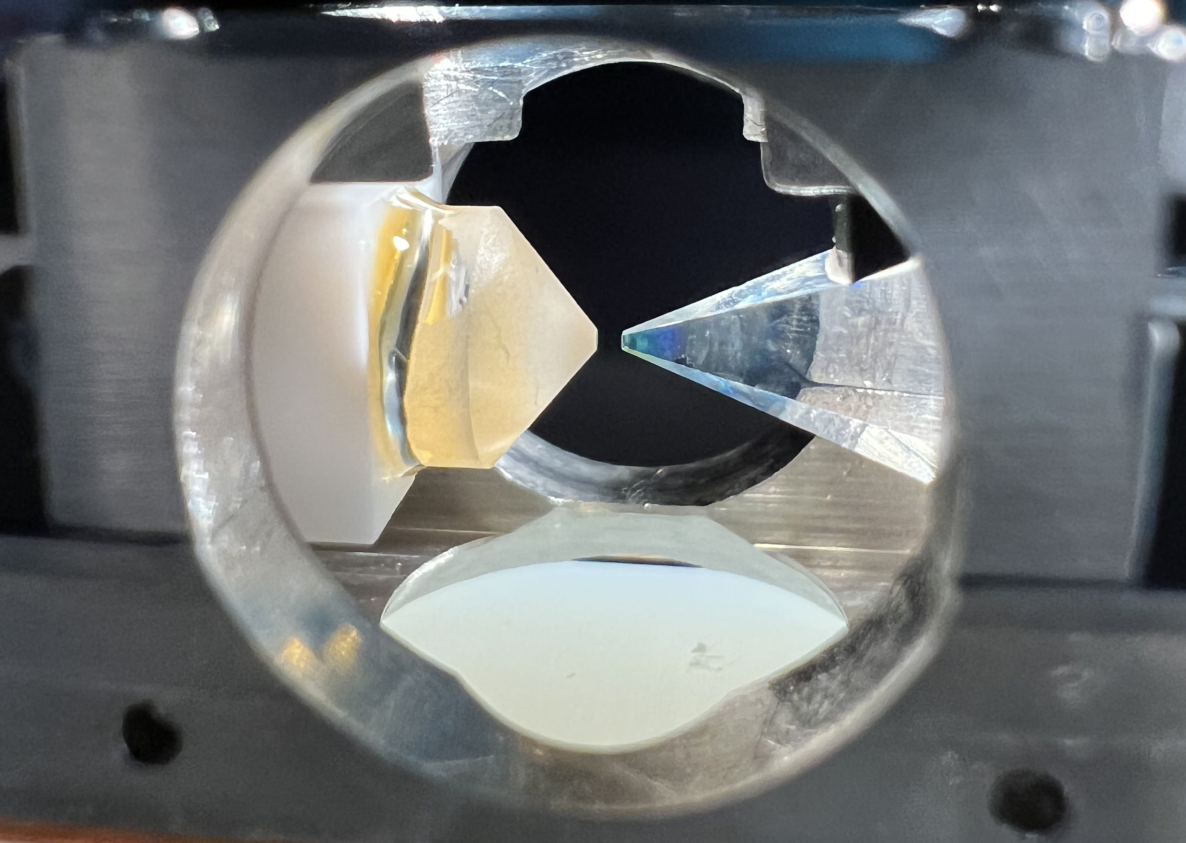
\includegraphics[width=6cm] {cavity.pdf}};;
		\end{tikzpicture}
		\centering
		\caption{}
		\label{b}
	\end{subfigure}
	\\
	\vspace{0.3em}
	\begin{subfigure}[b]{.49\linewidth}
		\begin{tikzpicture}
		\centering
		\node[inner sep=0] (image) {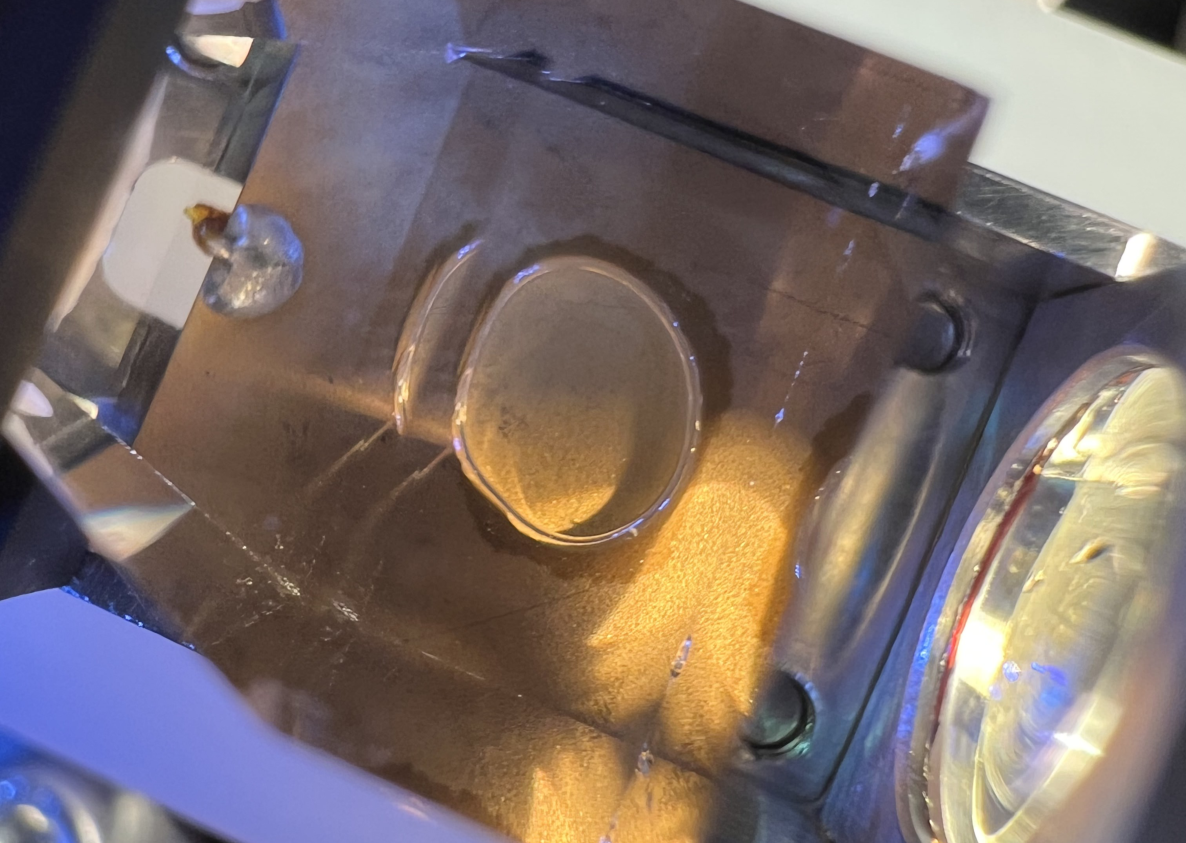
\includegraphics[width=6cm] {glue.pdf}};;
		\end{tikzpicture}
		\centering
		\caption{}
		\label{b}
	\end{subfigure}
	\begin{subfigure}[b]{.49\linewidth}
		\begin{tikzpicture}
		\centering
		\node[inner sep=0] (image) {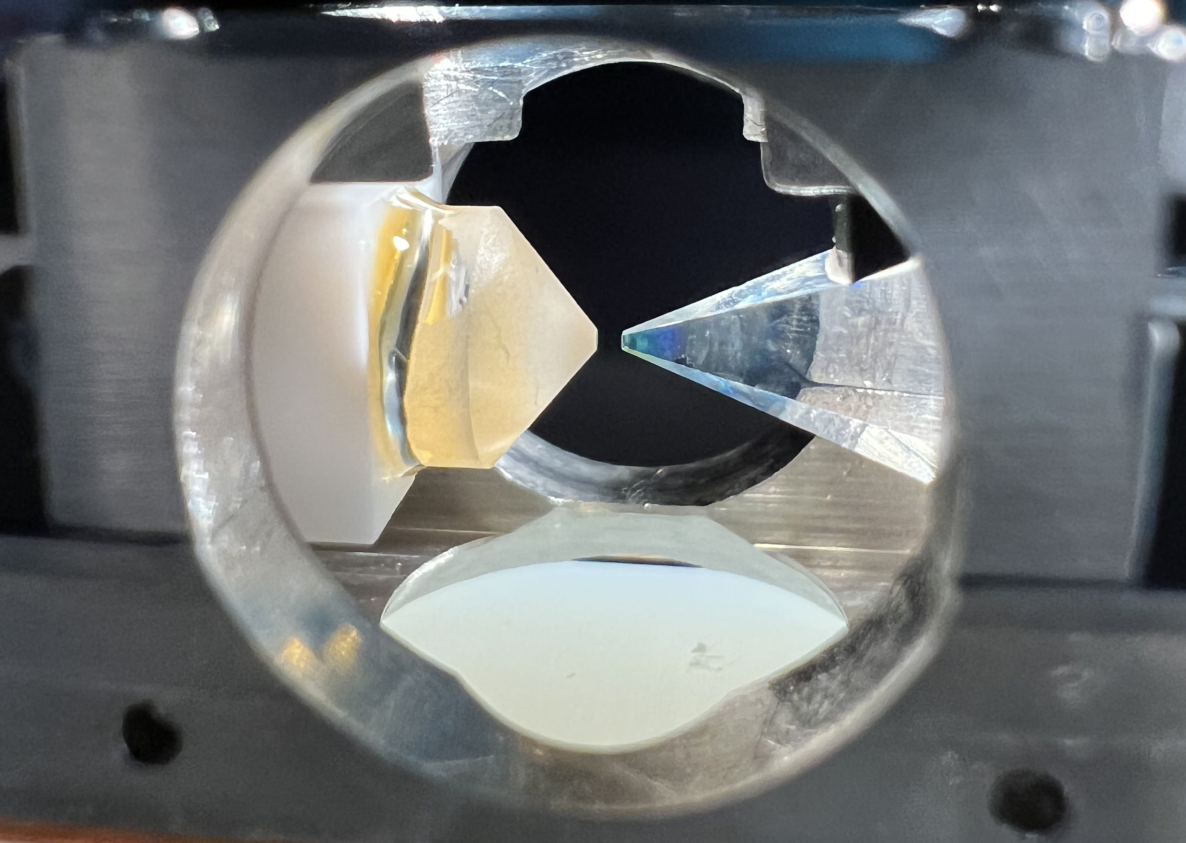
\includegraphics[width=6cm] {cavity.pdf}};;
		\end{tikzpicture}
		\centering
		\caption{}
		\label{b}
	\end{subfigure}
	\caption{(a) what is plotted is the log(10e-9 plus intensity)Recorded light intensity in the trapping plane. (b) Corresponding grid of optical power per trap in mW. (c) Integrated atom fluorescence. The box marks the 5 traps used for analysis of the ac-Stark shift (see \autoref{stark}). The $1/e^2$ diameter of the traps is $2.2\,\mu$m.}
	\label{asdf}
\end{figure}


\subsection{Mirror alignment}



\begin{figure}[t]
	\centering
	\begin{tikzpicture}
	\newcommand\step{0.157491}
	\newcommand\gap{0.0110096}
	
	\node[anchor=south west,inner sep=0] (image) at (0,0) {\includegraphics[width=0.85\textwidth]{{"all"}.pdf}};
	\begin{scope}[x={(image.south east)},y={(image.north west)}]
	
	%\draw[help lines,xstep=.1,ystep=.1] (0,0) grid (1,1);
	%\foreach \x in {0,1,...,9} { \node [anchor=north] at (\x/10,0) {0.\x}; }
	%\foreach \y in {0,1,...,9} { \node [anchor=east] at (0,\y/10) {0.\y}; }
	
	\draw[thick, ->, line cap=rect] (-0.012, 1.012) -- (-0.012, -0.02) node[above left] {$n_y$};
	\draw[thick, ->, line cap=rect] (-0.012, 1.012) -- (1.02, 1.012) node[above left] {$n_x$};
	
	\draw[thick, ->, line cap=rect] (0.661, 1-0.661) -- (1.02, 1-0.661) node[above left] {$n$};
	\draw[thick, ->, line cap=rect] (0.661, 1-0.661) -- (0.661, -0.02) node[above left] {$l$};
	
	\node[align=center] at (-0.03, \step/2) {$5$};
	\node[align=center] at (-0.03, 3*\step/2 + \gap) {$4$};
	\node[align=center] at (-0.03, 5*\step/2 + 2*\gap) {$3$};
	\node[align=center] at (-0.03, 7*\step/2 + 3*\gap) {$2$};
	\node[align=center] at (-0.03, 9*\step/2 + 4*\gap) {$1$};
	\node[align=center] at (-0.03, 11*\step/2 + 5*\gap) {$0$};
	
	\node[align=center] at (\step/2, 1.035) {$0$};
	\node[align=center] at (3*\step/2 + \gap, 1.035) {$1$};
	\node[align=center] at (5*\step/2 + 2*\gap, 1.035) {$2$};
	\node[align=center] at (7*\step/2 + 3*\gap, 1.035) {$3$};
	\node[align=center] at (9*\step/2 + 4*\gap, 1.035) {$4$};
	\node[align=center] at (11*\step/2 + 5*\gap, 1.035) {$5$};
	
	\node[align=center] at (0.661-0.018, 3*\step/2 + \gap) {$0$};
	\node[align=center] at (0.661-0.018, \step/2) {$1$};
	\node[align=center] at (0.661+0.012 + \step/2, 1-0.661+0.023) {$0$};
	\node[align=center] at (0.661+0.012 + 3*\step/2 + \gap, 1-0.661+0.023) {$1$};
	
	\end{scope}
	\end{tikzpicture}
	\caption[Optical setup for generation of dipole traps and MOT.]{(Left) Optical setup for the generation of \SI{1064}{\nano\meter} dipole traps and the detection of fluorescence. A spatial light modulator (SLM) generates a tweezer array inside the glass cell, monitored via a CCD. A dichroic mirror (DM) redirects the fluorescence into a detection path, where atoms are imaged using an EMCCD camera. Numbers indicate the beam magnification factors. (Right) Optical setup for the generation of the MOT inside a glass cell using $3$ retro-reflected beams. A pair of high-NA lenses focus and image the dipole trapping light.}
	\label{cavitymodes} 
\end{figure}


\section{Characterisation}

\subsection{Overview}

\subsection{Transverse modes}




\end{document}